\documentclass{article}[IEEEtran]
\usepackage[a4paper,
            left=1in,right=1in,top=1in,bottom=0.5in,
            footskip=.25in]{geometry}
\usepackage[utf8]{inputenc}
\usepackage{siunitx} % Provides the \SI{}{} and \si{} command for typesetting SI units
\usepackage{graphicx} % Required for the inclusion of images
\usepackage{amsmath} % Required for some math elements 
\usepackage{caption}
\usepackage{tikz}
\usepackage{import}
\usepackage{fancyhdr}
\usepackage[english]{babel}
\usepackage{algorithm}
\usepackage[noend]{algpseudocode}
\usepackage{pdfpages}
\usepackage{setspace}
\setlength\parindent{0pt} % Removes all indentation from paragraphs
\usepackage[export]{adjustbox}
\newcommand{\HRule}{\rule{\linewidth}{0.5mm}}
\usepackage{wrapfig}
\usepackage[font=scriptsize]{caption}
\usepackage{minted}
\usepackage{booktabs}
\usepackage{graphicx}

\renewcommand{\labelenumi}{\alph{enumi}.} % Make numbering in the enumerate environment by letter rather than number (e.g. section 6)

%\usepackage{times} % Uncomment to use the Times New Roman font

            
\pagestyle{fancy}
\pagenumbering{arabic}
\fancyhf{}
\fancyfoot[C]{\thepage}
\fancyhead[L]{\nouppercase SMBUD Project - Neo4j}


\usepackage{ifxetex}
\usepackage{ifluatex}
\newif\ifxetexorluatex % a new conditional starts as false
\ifnum 0\ifxetex 1\fi\ifluatex 1\fi>0
   \xetexorluatextrue
\fi

\ifxetexorluatex
  \usepackage{fontspec}
\else
  \usepackage[T1]{fontenc}
  \usepackage[utf8]{inputenc}
  \usepackage[lighttt]{lmodern}
\fi

\usepackage{textcomp}
\usepackage{xcolor}
\usepackage{listings}
\usepackage{upquote}

\definecolor{keyword}{HTML}{2771a3}
\definecolor{pattern}{HTML}{b53c2f}
\definecolor{string}{HTML}{be681c}
\definecolor{relation}{HTML}{7e4894}
\definecolor{variable}{HTML}{107762}
\definecolor{comment}{HTML}{8d9094}

\lstset{
	numbers=none,
	stepnumber=1,
	numbersep=5pt,
	basicstyle=\small\ttfamily,
	keywordstyle=\color{keyword}\bfseries\ttfamily,
	commentstyle=\color{comment}\ttfamily,
	stringstyle=\color{string}\ttfamily,
	identifierstyle=,
	showstringspaces=false,
	aboveskip=3pt,
	belowskip=3pt,
	columns=flexible,
	keepspaces=true,
	breaklines=true,	
	captionpos=b,
	tabsize=2,
	frame=none,
}

\lstset{upquote=true}

\lstdefinelanguage{cypher}
{
	morekeywords={
		MATCH, OPTIONAL, WHERE, NOT, AND, OR, XOR, RETURN, DISTINCT, ORDER, BY, ASC, ASCENDING, DESC, DESCENDING, UNWIND, AS, UNION, WITH, ALL, CREATE, DELETE, DETACH, REMOVE, SET, MERGE, SET, SKIP, LIMIT, IN, CASE, WHEN, THEN, ELSE, END,
		INDEX, DROP, UNIQUE, CONSTRAINT, EXPLAIN, PROFILE, START, COUNT, SUM, LOAD, CSV, FROM, HEADERS, WITH, date(, duration, datetime(), between( , true, false, FIELDTERMINATOR, Person, City, Place, Vaccine, Test, State, TOOK, WENT_TO, RECEIVED, LIVES_WITH, LIVES_IN, MET, LOCATED, PART_OF,
	}
}


\newcommand{\mycdots}{\cdot\!\cdot\!\cdot}
\lstset{language=cypher,
	literate=*
	{...}{$\mycdots$}{1}
	{theta}{$\theta$}{1}
}


\begin{document}
%===========================================================
\begin{titlepage}
\begin{center}

\captionsetup{font=footnotesize}

% Top 
\textsc{AY 2021-2022}\\[2cm]


\includegraphics[width=0.55\textwidth]{logo.png}~\\[2cm]


% Title
\HRule \\[0.4cm]
{ \LARGE 
  \textbf{SMBUD Project}\\[0.4cm]
  \emph{Covid Tracing-Oriented Neo4j Database}\\[0.4cm]
}
\HRule \\[1.5cm]



% Author
\begin{center}
    {\large Pablo Giaccaglia - 10626428\\[0.1cm]  Santi Pier Pistone - 10867402 \\[0.1cm]    Salvatore Cassata - 10560790\\[0.1cm]  Stefano Vighini - 10622788\\[0.1cm]  Zhitao He - 10763530\\[0.1cm] 
}
\end{center}

\vfill

\textsc{\large Master of Science in \\Computer Science \& Engineering}\\[0.4cm]


% Bottom
{\large \today}
 
\end{center}
\end{titlepage}

\newpage


%===========================================================
\tableofcontents
\addtocontents{toc}{\protect\thispagestyle{empty}}
\newpage
\setcounter{page}{1}

%===========================================================
%===========================================================
\section{Introduction}\label{sec:intro}

Considering the scenario in which there’s the need to build a system for managing the \textbf{COVID-19 pandemic} in a specific country, our project focuses on the data perspective level. This is why we designed and implemented a \textbf{Neo4j} \cite{neo4j2012world} data structure to face the need of contact tracing functionality, to monitor the viral diffusion. 


\section{Specification \& Hypothesis}\label{sec:spec-hyp}

The usage of this application involves the following actors :
\begin{itemize}
\item \textbf{normal citizens}, who get in touch with each other
\item \textbf{workers}, who need to trace part of the contacts
\end{itemize}
and the following devices :
\begin{itemize}
\item a \textbf{server} storing a database (which could evolve in a distributed system, with every country having its own database)
\item \textbf{devices} such as smartphones or wearable, which can use Bluetooth and store a simple script, and have an internet connection (or can communicate to a device with it).
\end{itemize}

The purpose of this project is to track the spread of \textbf{COVID-19}. The first design choice concerning the database records it's indeed about tracking. 
There are mainly 2 ways to do it:
\begin{itemize}

\item \textbf{automatically} (with smartphones or wearables): we suppose that, depending on the country, we might have different applications or technologies that keep track of the fact that people occasionally are in the same place at the same time, so the system is designed to also store contact tracing app data. This type of contact tracking is represented by the \textbf{MET} relationship.

\item \textbf{manually} (explicit data collection): data coming from specific locations, such as restaurants, theaters or hospitals, that explicitly record people’s presence, asking them personal information.  This type of contact tracking is represented by the \textbf{WENT TO} relationship

\end{itemize}

We could have used the \textbf{MET} relationship in both cases, but this division leads to a less redundant database. For example, if 100 people go in the same place on a certain date, $100^{2}$ relationships between people should be stored if there wasn't a \textbf{WENT TO} relationship. In this way instead, only 100 relationships are needed, resulting in a way lighter database.
\\ \\
We also chose to have \textbf{Vaccines} and \textbf{Tests} as entities and to store the information about date, number, vaccination city and result in the corresponding relationships. This choice doesn't really make the difference, as we could also have kept this information in the entities. Anyways, for future use there could be the need to store additional information in vaccines and tests, so we made this choice to avoid redundancy.
\\\\
The relationships' names \textbf{RECEIVED} and \textbf{TOOK} have to be interpreted along with Vaccine and Test, as this DB is only for pandemic purposes, so these have an unique meaning.
\\
We also numbered the vaccines taken in the RECEIVED relationship to have quicker queries, as it could be an useful information to extract, in addition to being a much more efficient design choice than determining it through queries.
\\ \\


\section{Data Model (ER Diagram)}\label{sec:data}

\begin{figure}[H]
\begin{center}
    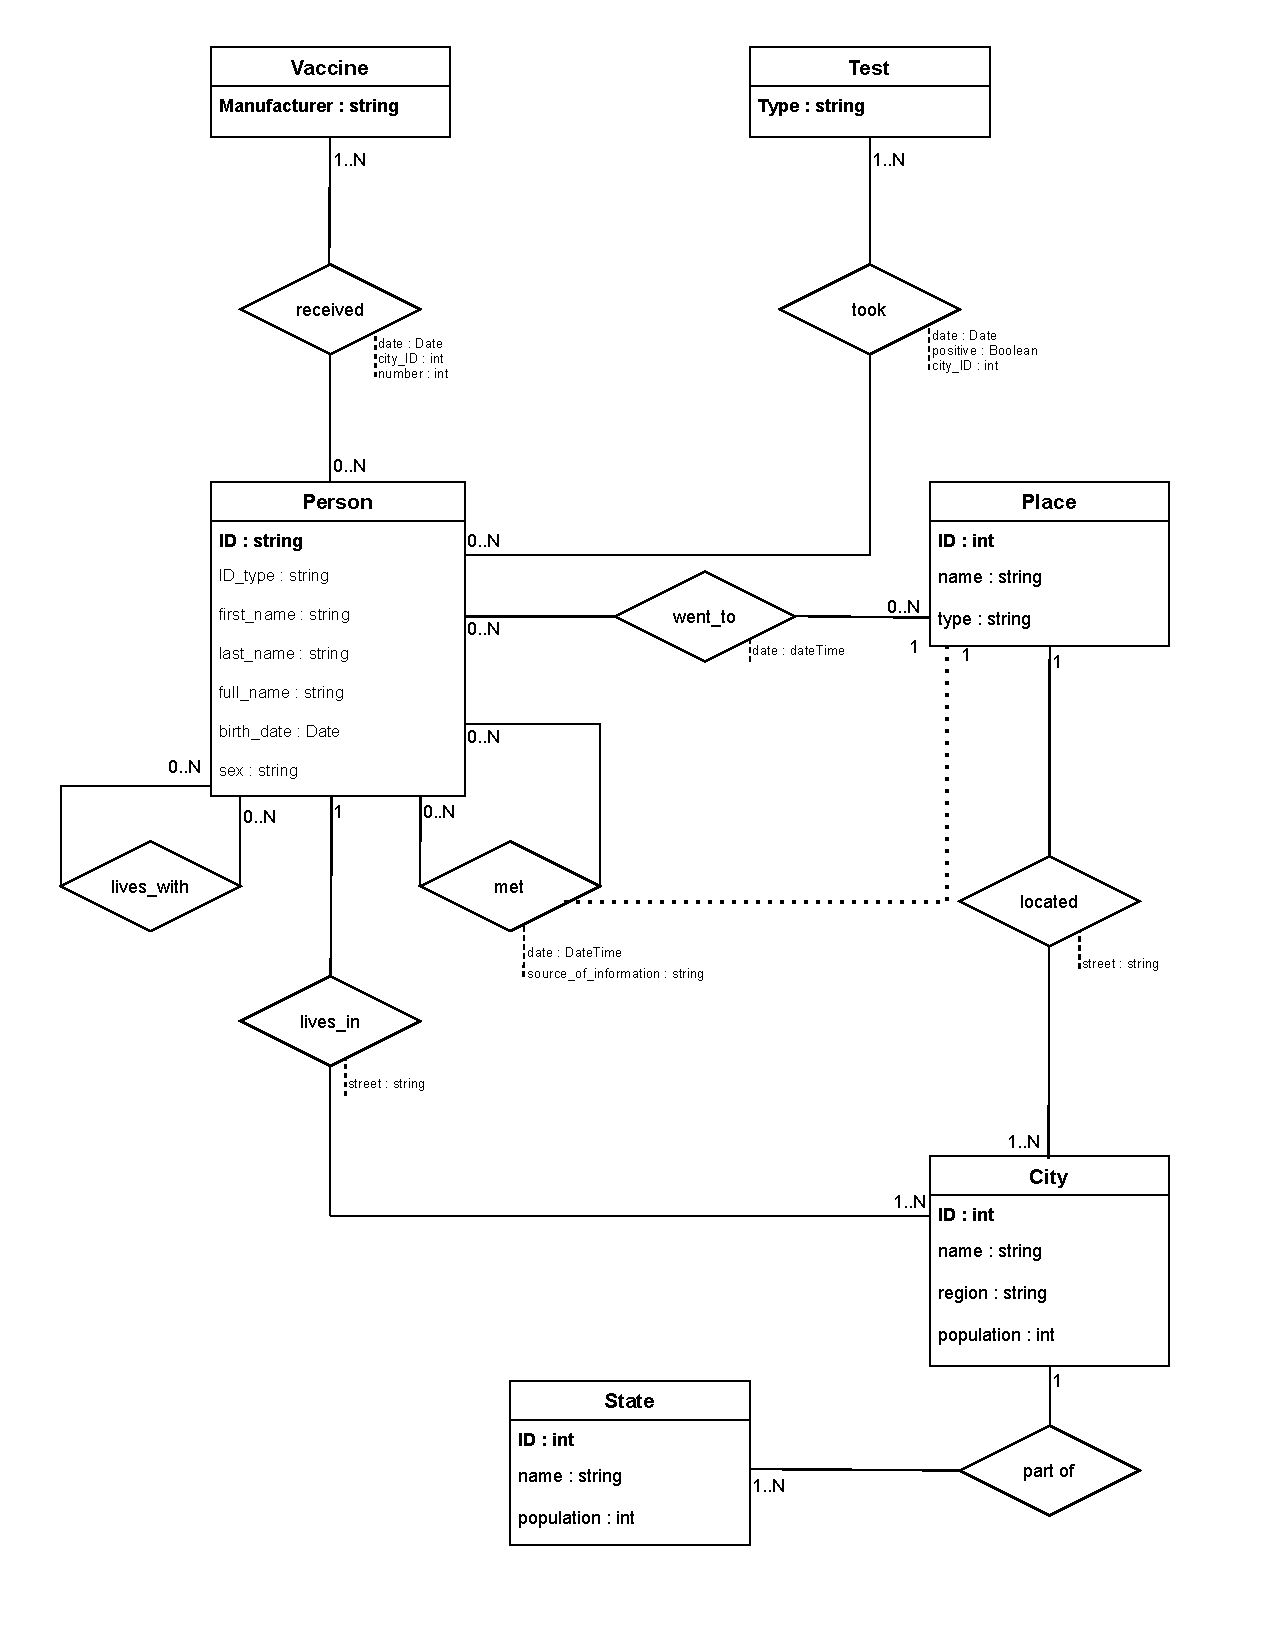
\includegraphics[width=\textwidth]{ER_Neo4J.pdf}
    \caption{ER Diagram}
\end{center}
\end{figure}

\newpage

The model's entities are:

\begin{itemize}
\item \textbf{People}: each person has a corresponding node in the database with its own features (attributes) which are :
    \begin{itemize}
    \item Personal Recognition Document ID
    \item Personal Recognition Document Type
    \item First Name
    \item Last Name
    \item Full Name
    \item Birth Date
    \item Sex
    \end{itemize}
    
\item \textbf{Covid vaccines}: each vaccine manufacturer has a corresponding node in the database with its own features (attributes), which are :
\begin{itemize}
\item Manufacturer Name
\end{itemize}

\item \textbf{Covid tests}: each test typology has a corresponding node in the database with its own features (attributes), which are :
\begin{itemize}
\item Test Type \{Molecular test/Antigen test/Antibody test\}
\end{itemize}

\item \textbf{Places}: each place has a corresponding node in the database with its own features (attributes), which are :
\begin{itemize}
\item Place ID
\item Name
\item Type \{restaurant/cafe/theater/cinema/hospital\}
\end{itemize}

\item \textbf{Cities}: each city has a corresponding node in the database with its own features (attributes), which are :
\begin{itemize}
\item City ID
\item Name
\item Region
\item Population amount
\end{itemize}

\item \textbf{States}: each state has a corresponding node in the database with its own features (attributes), which are :
\begin{itemize}
\item State ID
\item Name
\item Population amount
\end{itemize}


\end{itemize}

The data retrieval process to populate the database with these entities and further clarifications is explained in section 4. Along with these nodes, the Neo4j database is composed by several relationships, illustrated in the following section and in section 3, where there is a brief in-depth explanation for each one.


\newpage
\subsection{Relationships}

Several types of relationships are stored in the system. The following sections illustrate their visual representation taken from the \textbf{Neo4j Bloom} \cite{neo4jbloom} graph exploration application followed by a \\ brief explanation.

It is important to point out that \textbf{"undirected"} relationships are intended to be \textbf{symmetrical} \\ (e.g "MET RELATIONSHIP" : for every P1 that met P2, also P2 met P1), even though Neo4j \\ doesn't explicitly allows to have them, but allows to have the notion of undirected edges at query time\cite{neo4jundirected}.

\vspace{0.5cm}


\subsubsection{RECEIVED}

\begin{wrapfigure}[14]{R}{0.43\textwidth}
\vspace{-1.5cm}
\begin{center}
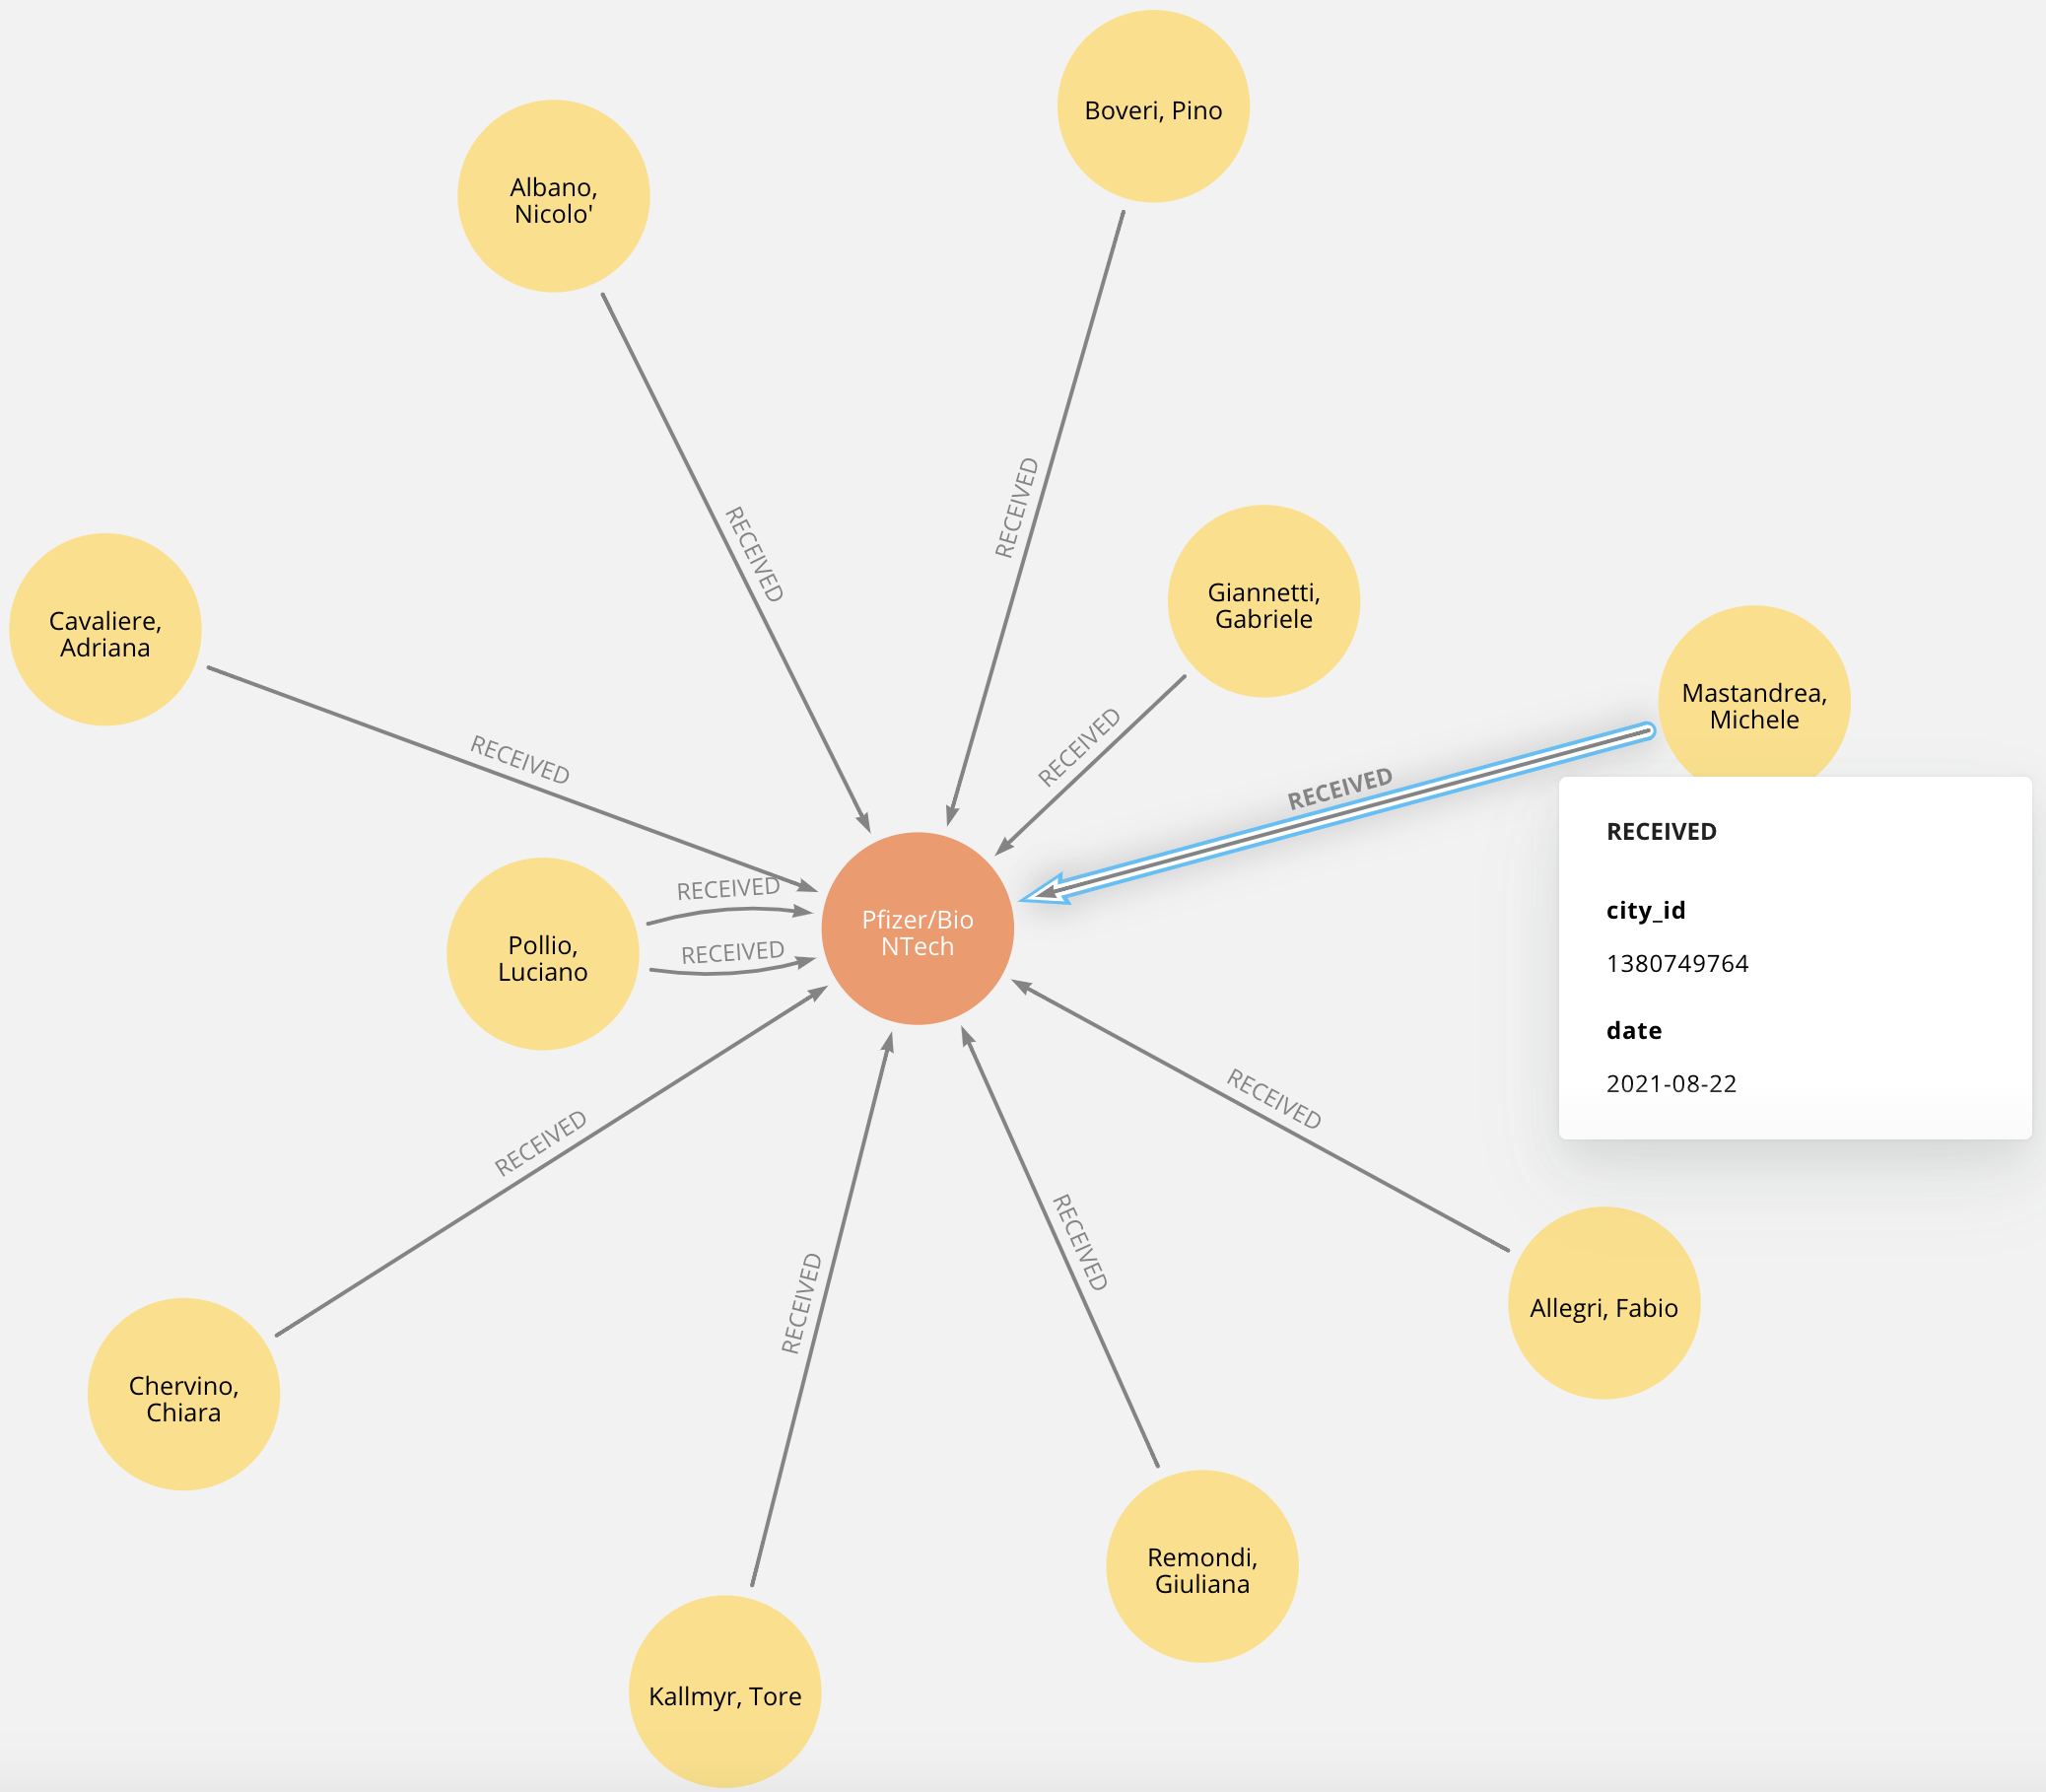
\includegraphics[width=0.55\textwidth, frame]{RECEIVED.png}
\caption{\emph{"RECEIVED"} Relationship Visualization}
\end{center}
\end{wrapfigure}
This directed relationship connects a \textbf{Person} node to a \textbf{Covid Vaccine}. Multiple RECEIVED relationships  can exists for the same person, indicating the fact that he/she has received multiple Covid vaccine doses of the same manufacturer. In our sample dataset each \textbf{Person} node is associated with  at most 2 \emph{"RECEIVED"} relationships.
\\\\
The connection stores the following attributes:
\begin{itemize}
    \item Date of the vaccination \\ (\textbf{ranging from 2021-01-05 to 2021-11-7})
    \item The city of the vaccination
    \item The number of vaccination dose.
\end{itemize}

\vspace{2cm}


\subsubsection{TOOK}

\begin{wrapfigure}[14]{R}{0.43\textwidth}
\vspace{-1.5cm}
\begin{center}
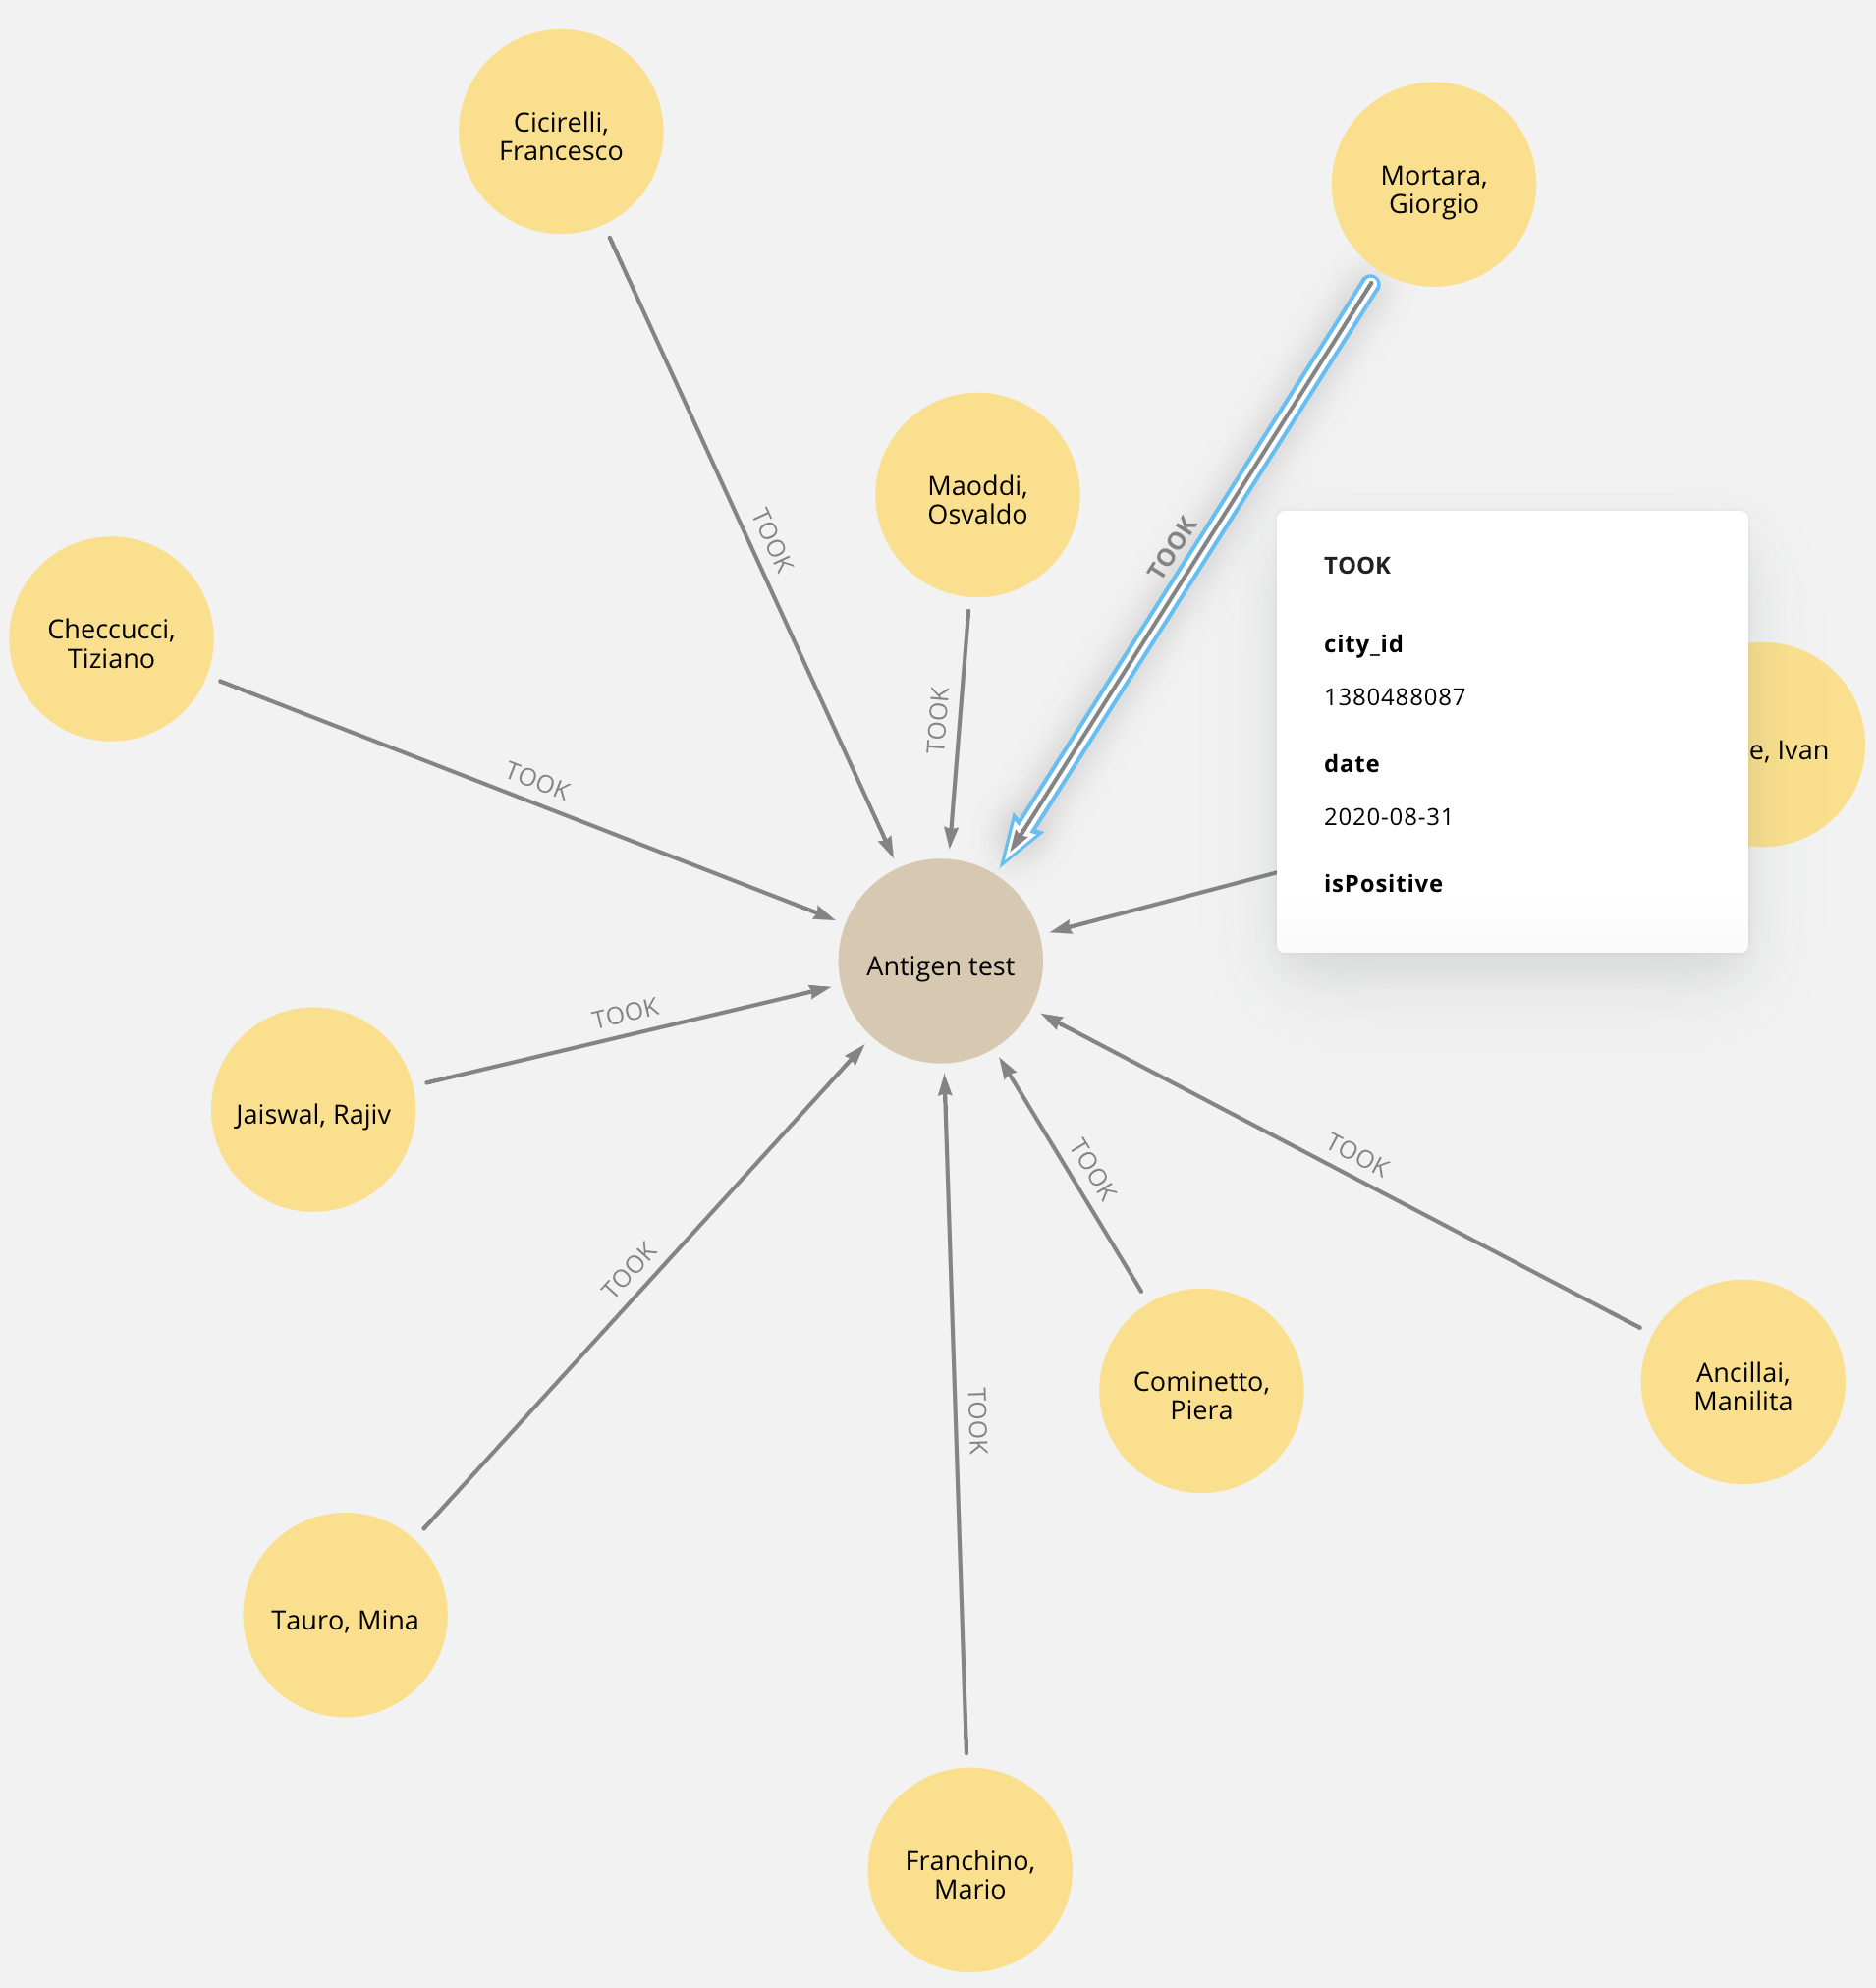
\includegraphics[width=0.55\textwidth, frame]{TOOK.png}
\caption{\emph{"TOOK"} Relationship Visualization}
\end{center}
\end{wrapfigure}

This directed relationship connects a \textbf{Person} node to a \textbf{Covid Test} node. Multiple TOOK relationship can exists for the same person, indicating the fact that he/she has done multiple tests. In our sample dataset each \textbf{Person} node is associated with at most 4 \emph{"TOOK"} relationships.
\\\\
The connection stores the following attributes:
\begin{itemize}
    \item Date of the test \\ (\textbf{ranging from 2020-03-10 to 2021-11-07})
    \item The city where the test has been taken
    \item The outcome of the test \{\textbf{Positive/Negative}\}
\end{itemize}

\newpage

\subsubsection{WENT TO}

This directed relationship connects a \textbf{Person} node to a \textbf{Place} node.
If the database contains such information it means that there has been an explicit manual registration from specific locations, such as restaurants, theaters or hospitals, that explicitly record people’s presence, asking them for their names. In our sample dataset, each \textbf{Person} node is associated with exactly 50 \emph{"WENT TO"} \\ relationships.
\\\\
The connection stores the following attributes:
\begin{itemize}
\item Date of the registration (\textbf{ranging from 2020-3-10 to 2021-11-07})
\end{itemize}

\begin{figure}[H]
\begin{center}
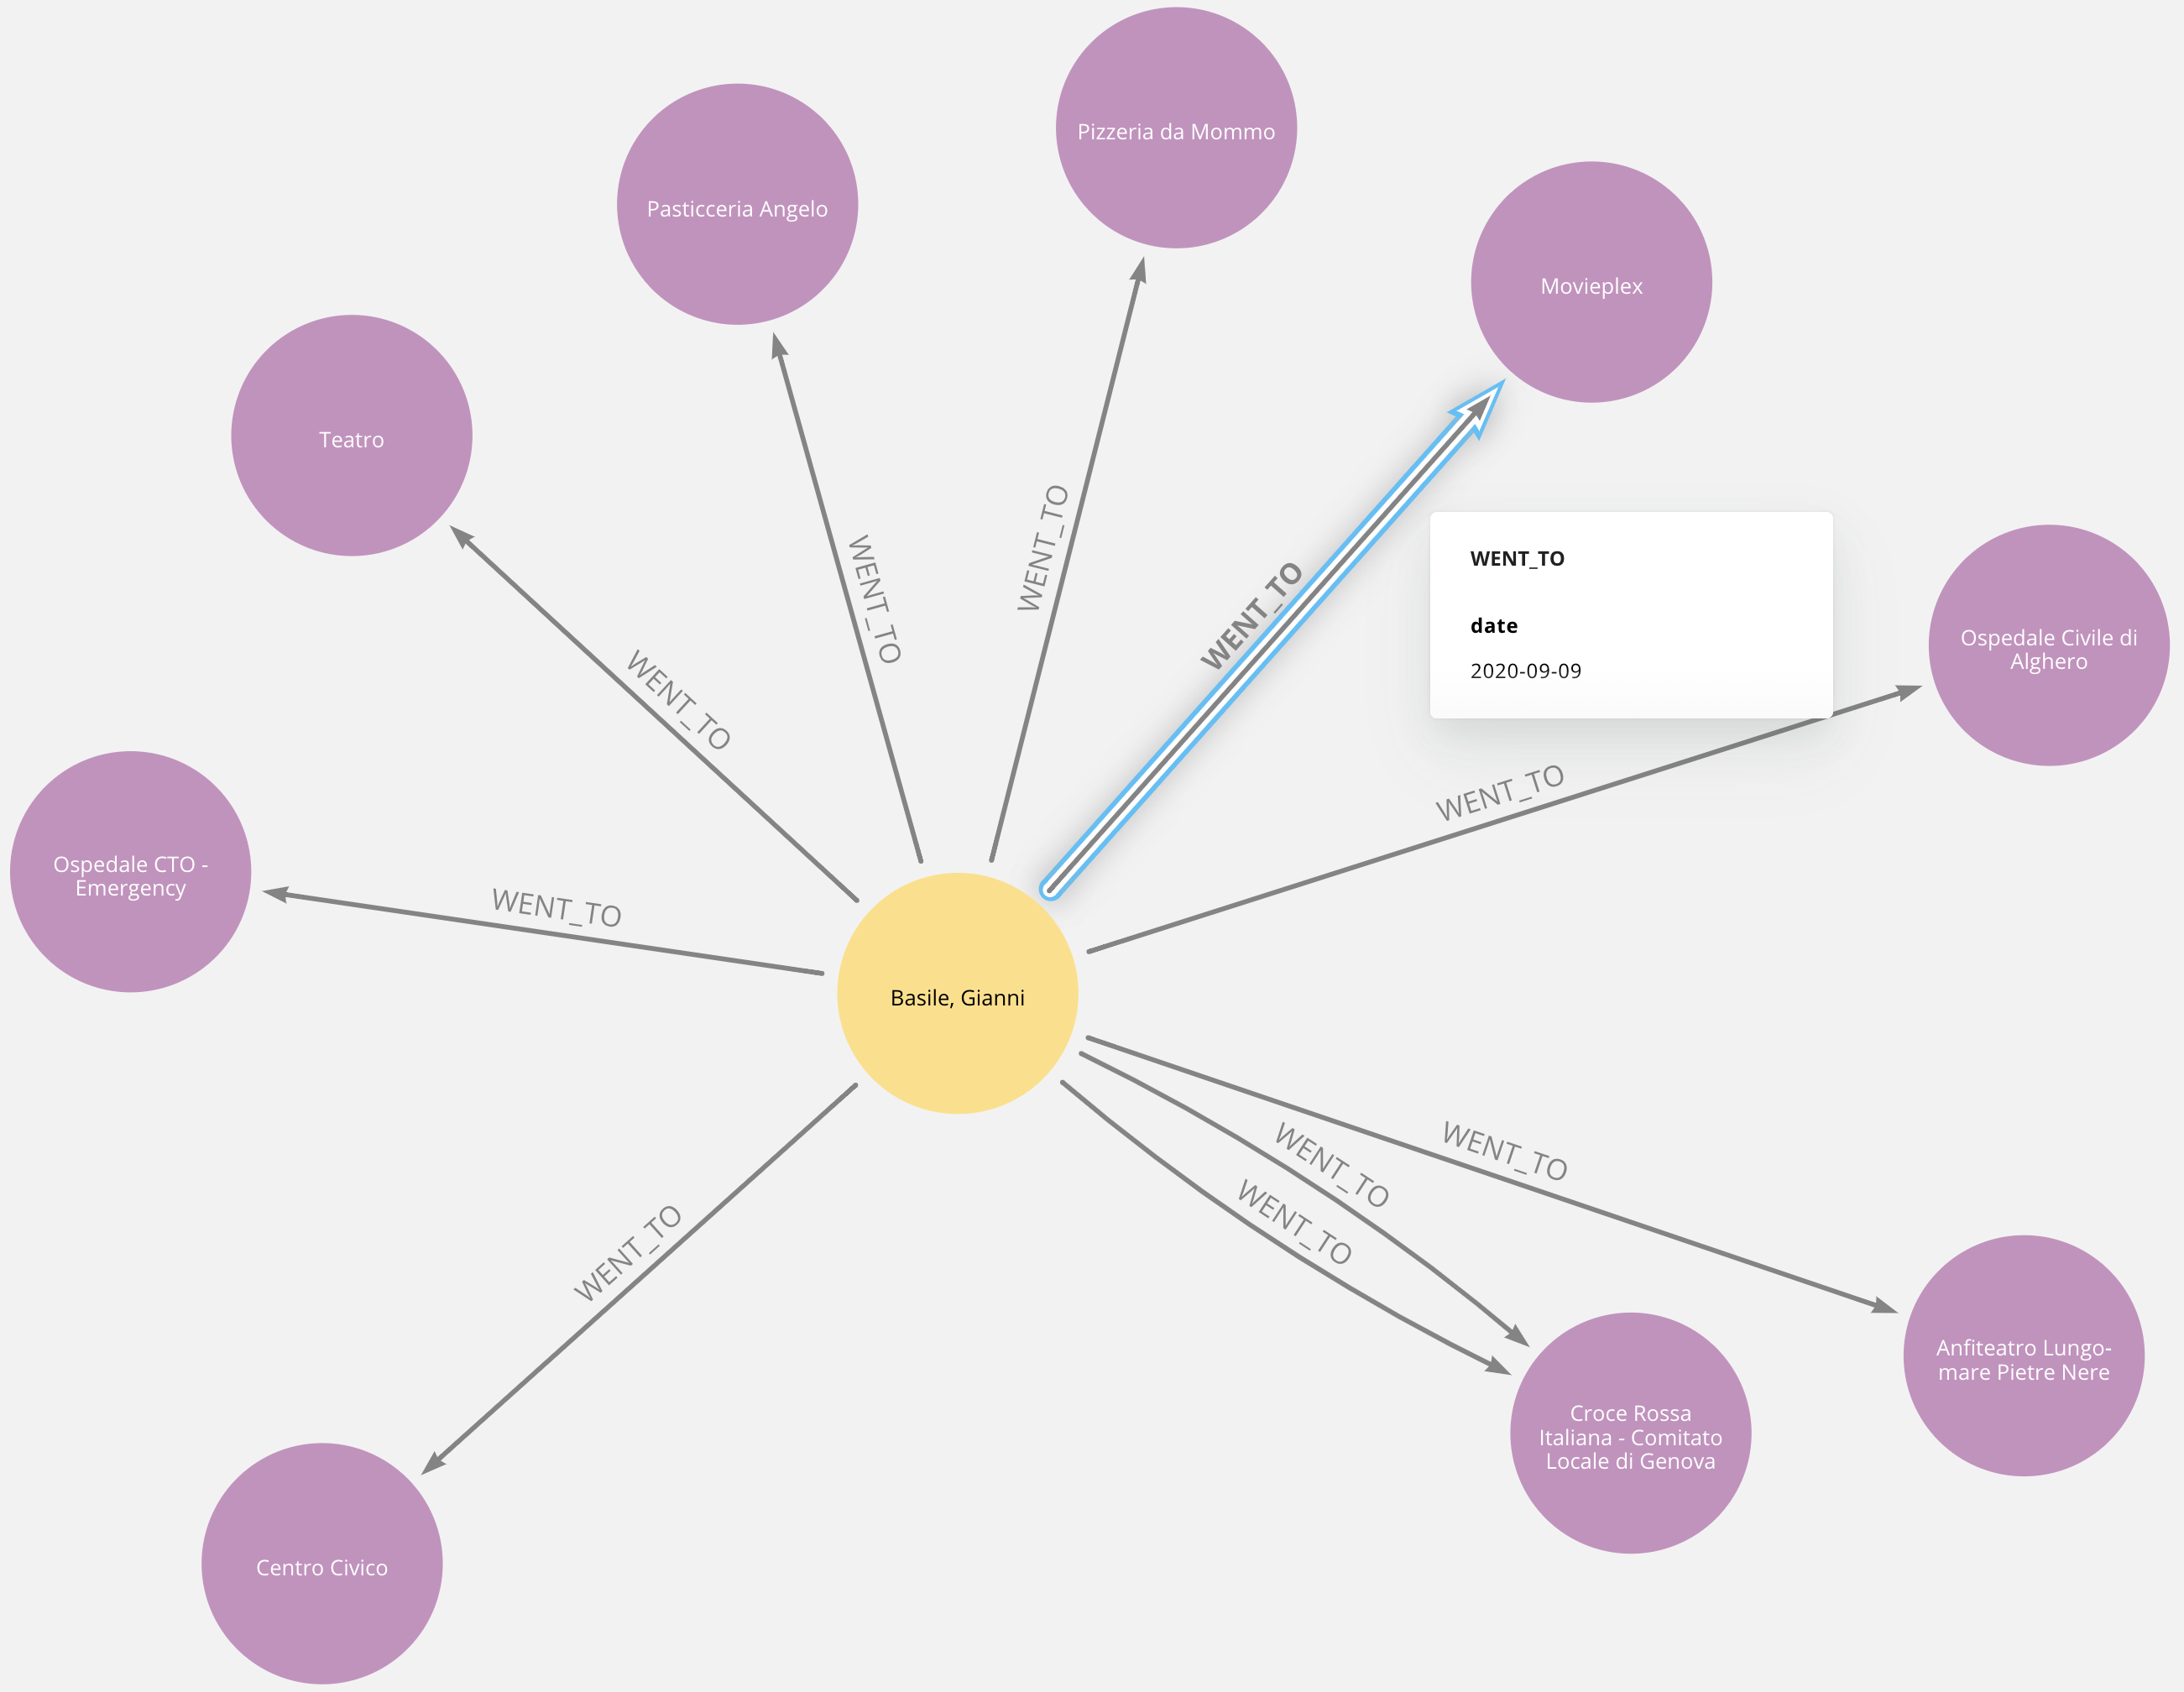
\includegraphics[width=0.56\linewidth, frame]{WENT_TO.png}
\caption{\emph{"WENT TO"} Relationship Visualization}
\end{center}
\end{figure}

\subsubsection{LIVES WITH}

This undirected relationship connects two \textbf{Person} nodes. 
Every pair of people who belong to the same family or live in the same house are considered \textbf{always} in touch. The assumption is that we don’t want the tracing system to be recording every second contact of people living together, so they are in contact by default. In our sample dataset each \textbf{Person} node is associated with at most 6 \emph{"LIVES WITH"} \\ relationships.
The connection doesn't store attributes.

\begin{figure}[H]
\begin{center}
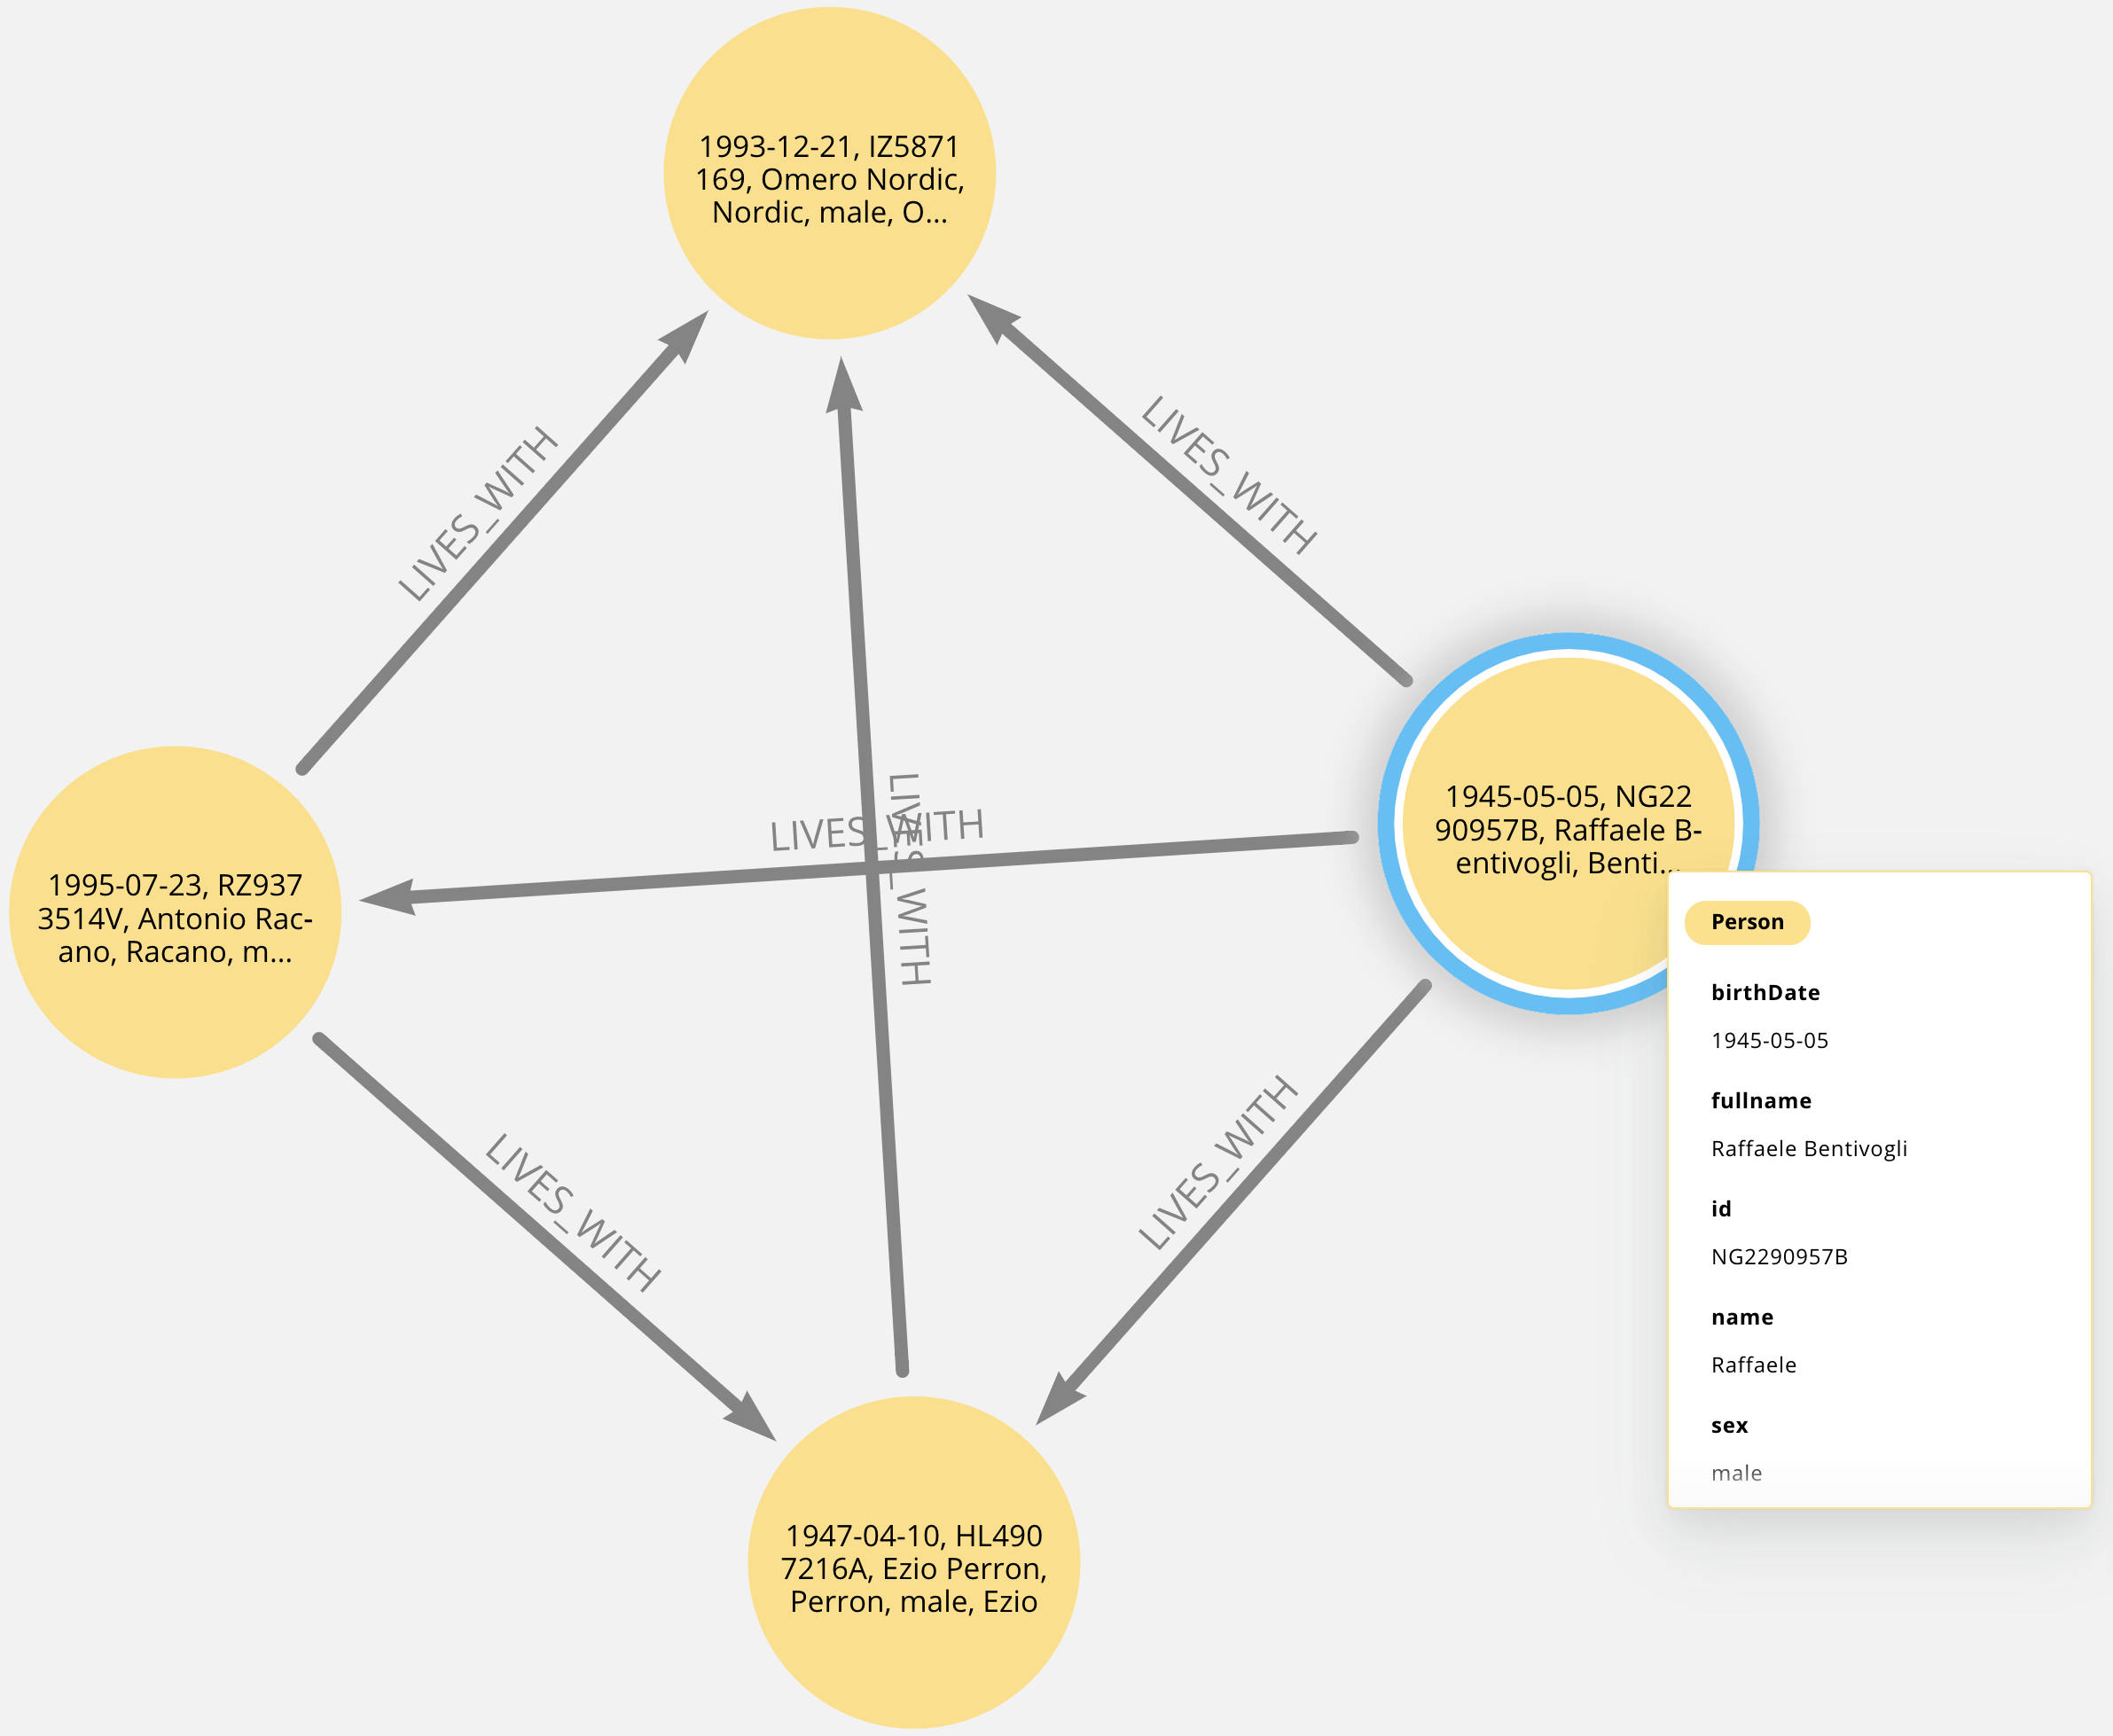
\includegraphics[width=0.56\linewidth, frame]{LIVES_WITH.png}
\caption{\emph{"LIVES WITH"} Relationship Visualization}
\end{center}
\end{figure}

\newpage 

\subsubsection{LIVES IN}

\begin{wrapfigure}[8]{R}{0.4 \textwidth}
\vspace{-1.5cm}
\begin{center}
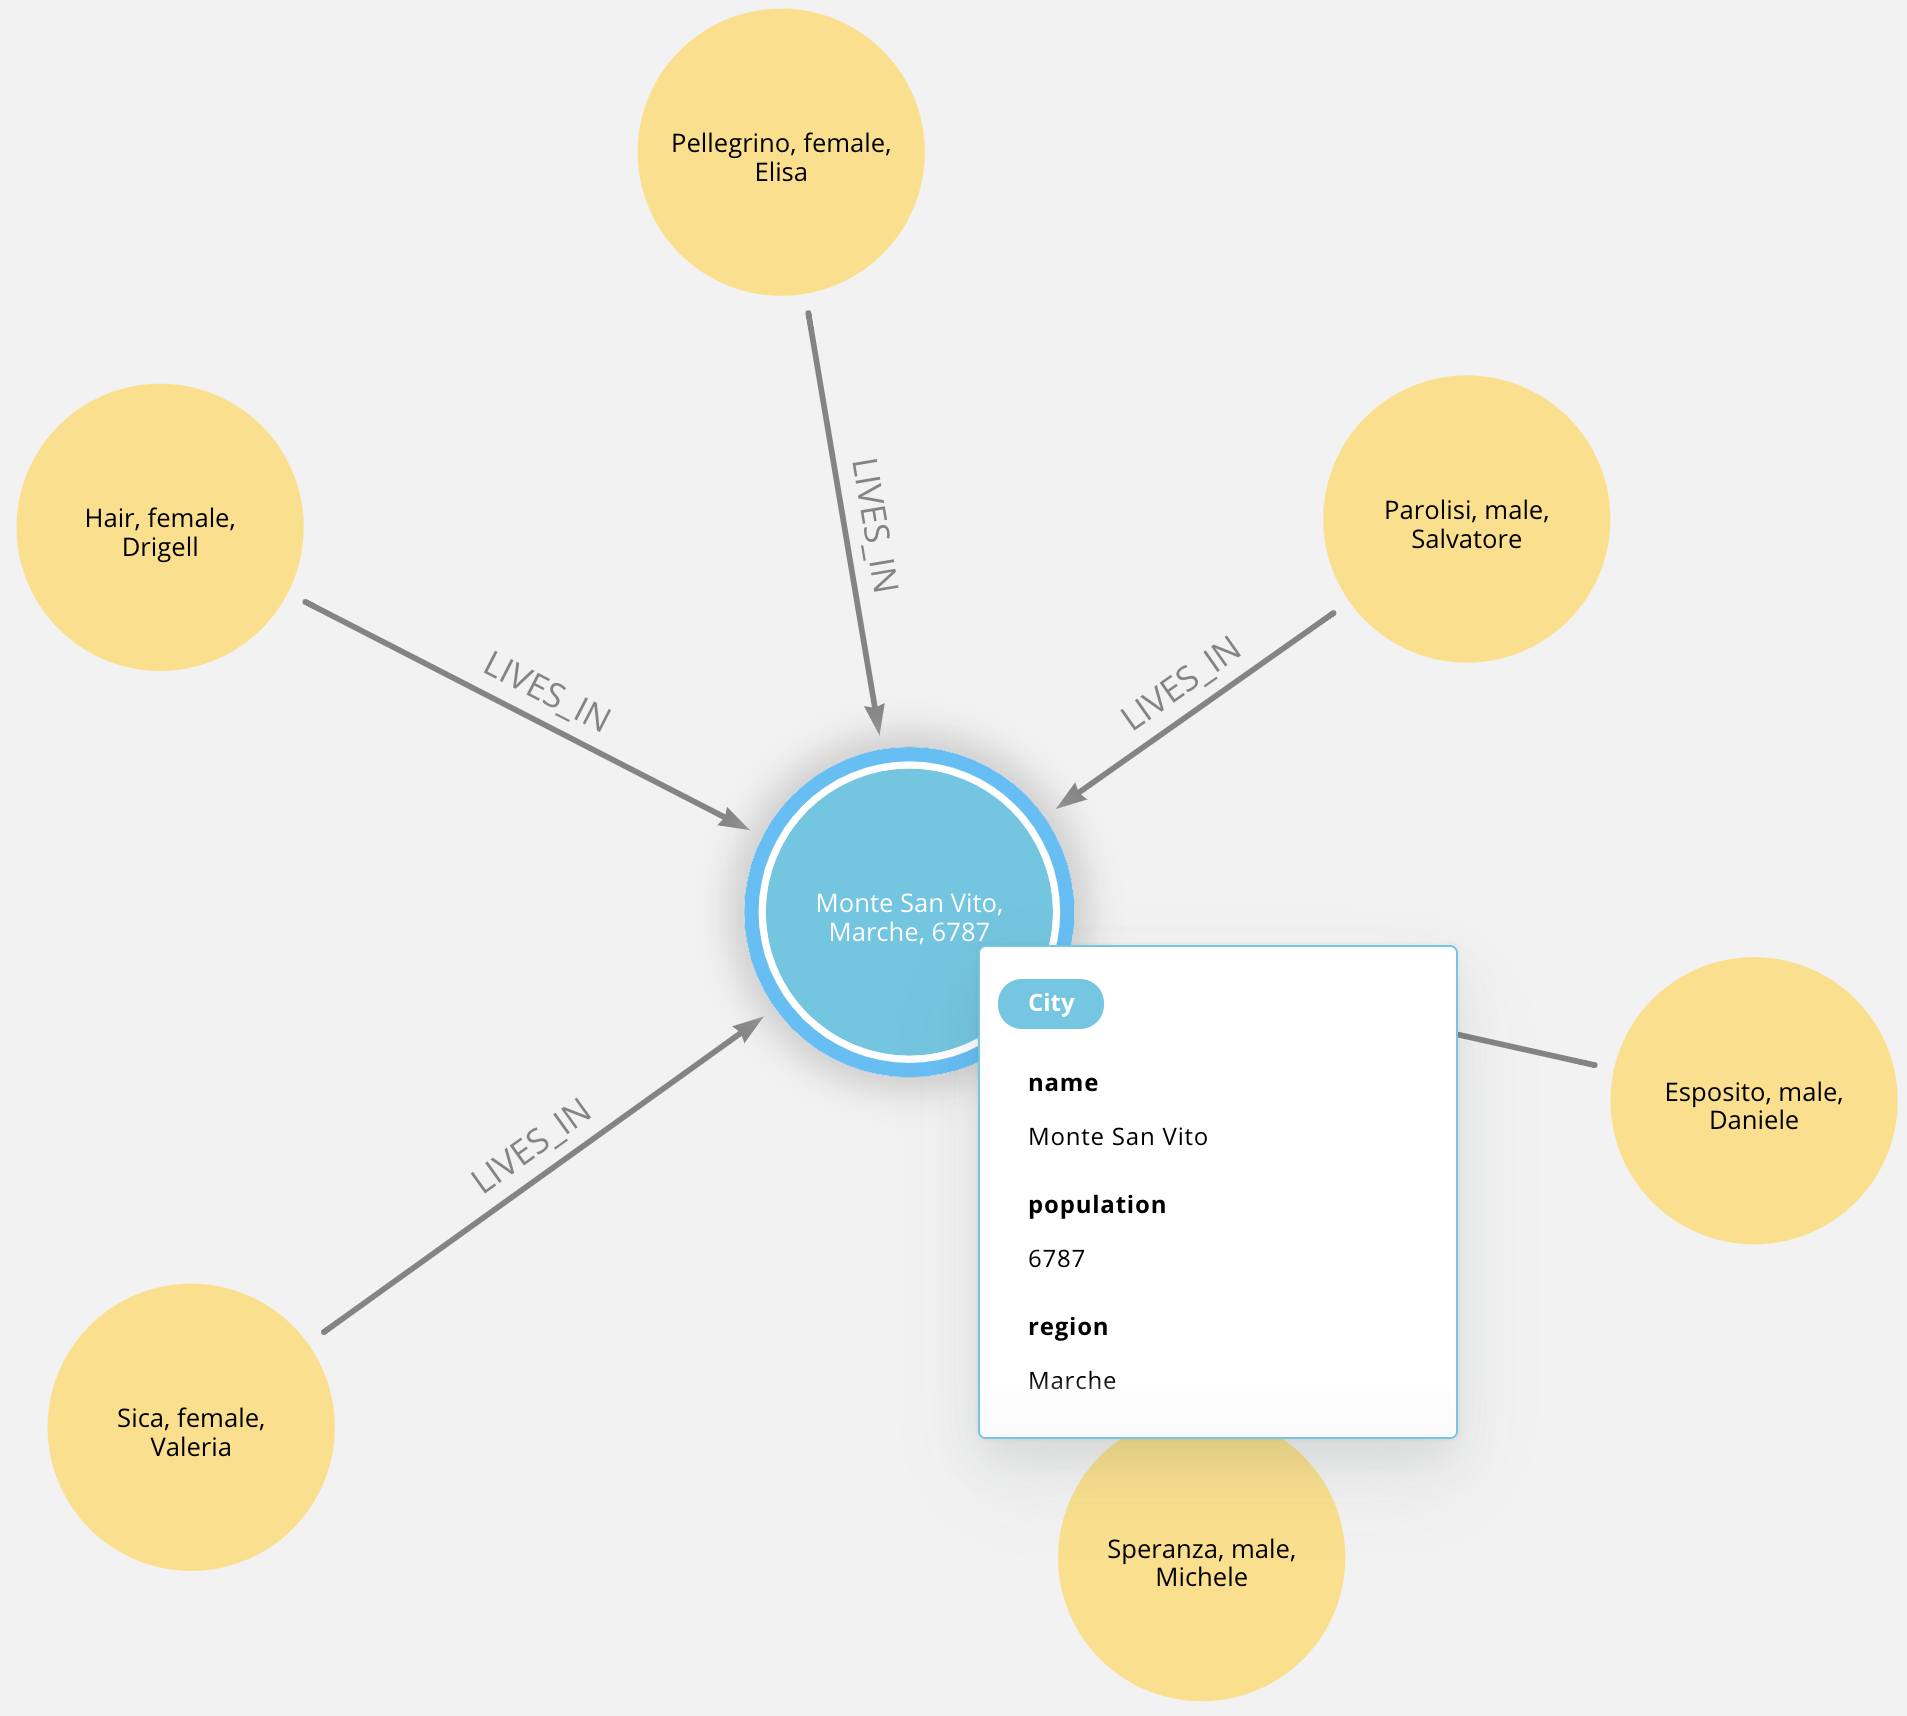
\includegraphics[width=0.55\textwidth, frame]{LIVES_IN.png}
\caption{\emph{"LIVES IN"} Relationship Visualization}
\end{center}
\end{wrapfigure}

This directed relationship connects a \textbf{Person} node to a \textbf{City} node. We assume that each \textbf{Person} node is associated with exactly one \\\emph{"LIVES IN"} relationship.
\\\\
The connection stores the following attributes:
\begin{itemize}
    \item Address of the residence
\end{itemize}

\vspace{4cm}

\subsubsection{MET}

This undirected relationship connects two \textbf{Person} nodes. This information comes from contact tracing app or technologies that keep track of the fact that people occasionally are in the same place at the same time. We assume that the technologies providing this information don't keep track of the location of the contact. In our sample dataset each \textbf{Person} node is associated with a number of \emph{"MET} relationships ranging from 10 to 50 (inclusive).
\\\\
The connection stores the following attributes:
\begin{itemize}
    \item Date of the contact (\textbf{ranging from 2020-03-10 to 2021-11-07})
    \item Source of tracking info \{e.g \textbf{Smartphone/Smartwatch/Tracking Wearable}\}
\end{itemize}


\begin{figure}[H]
\begin{center}
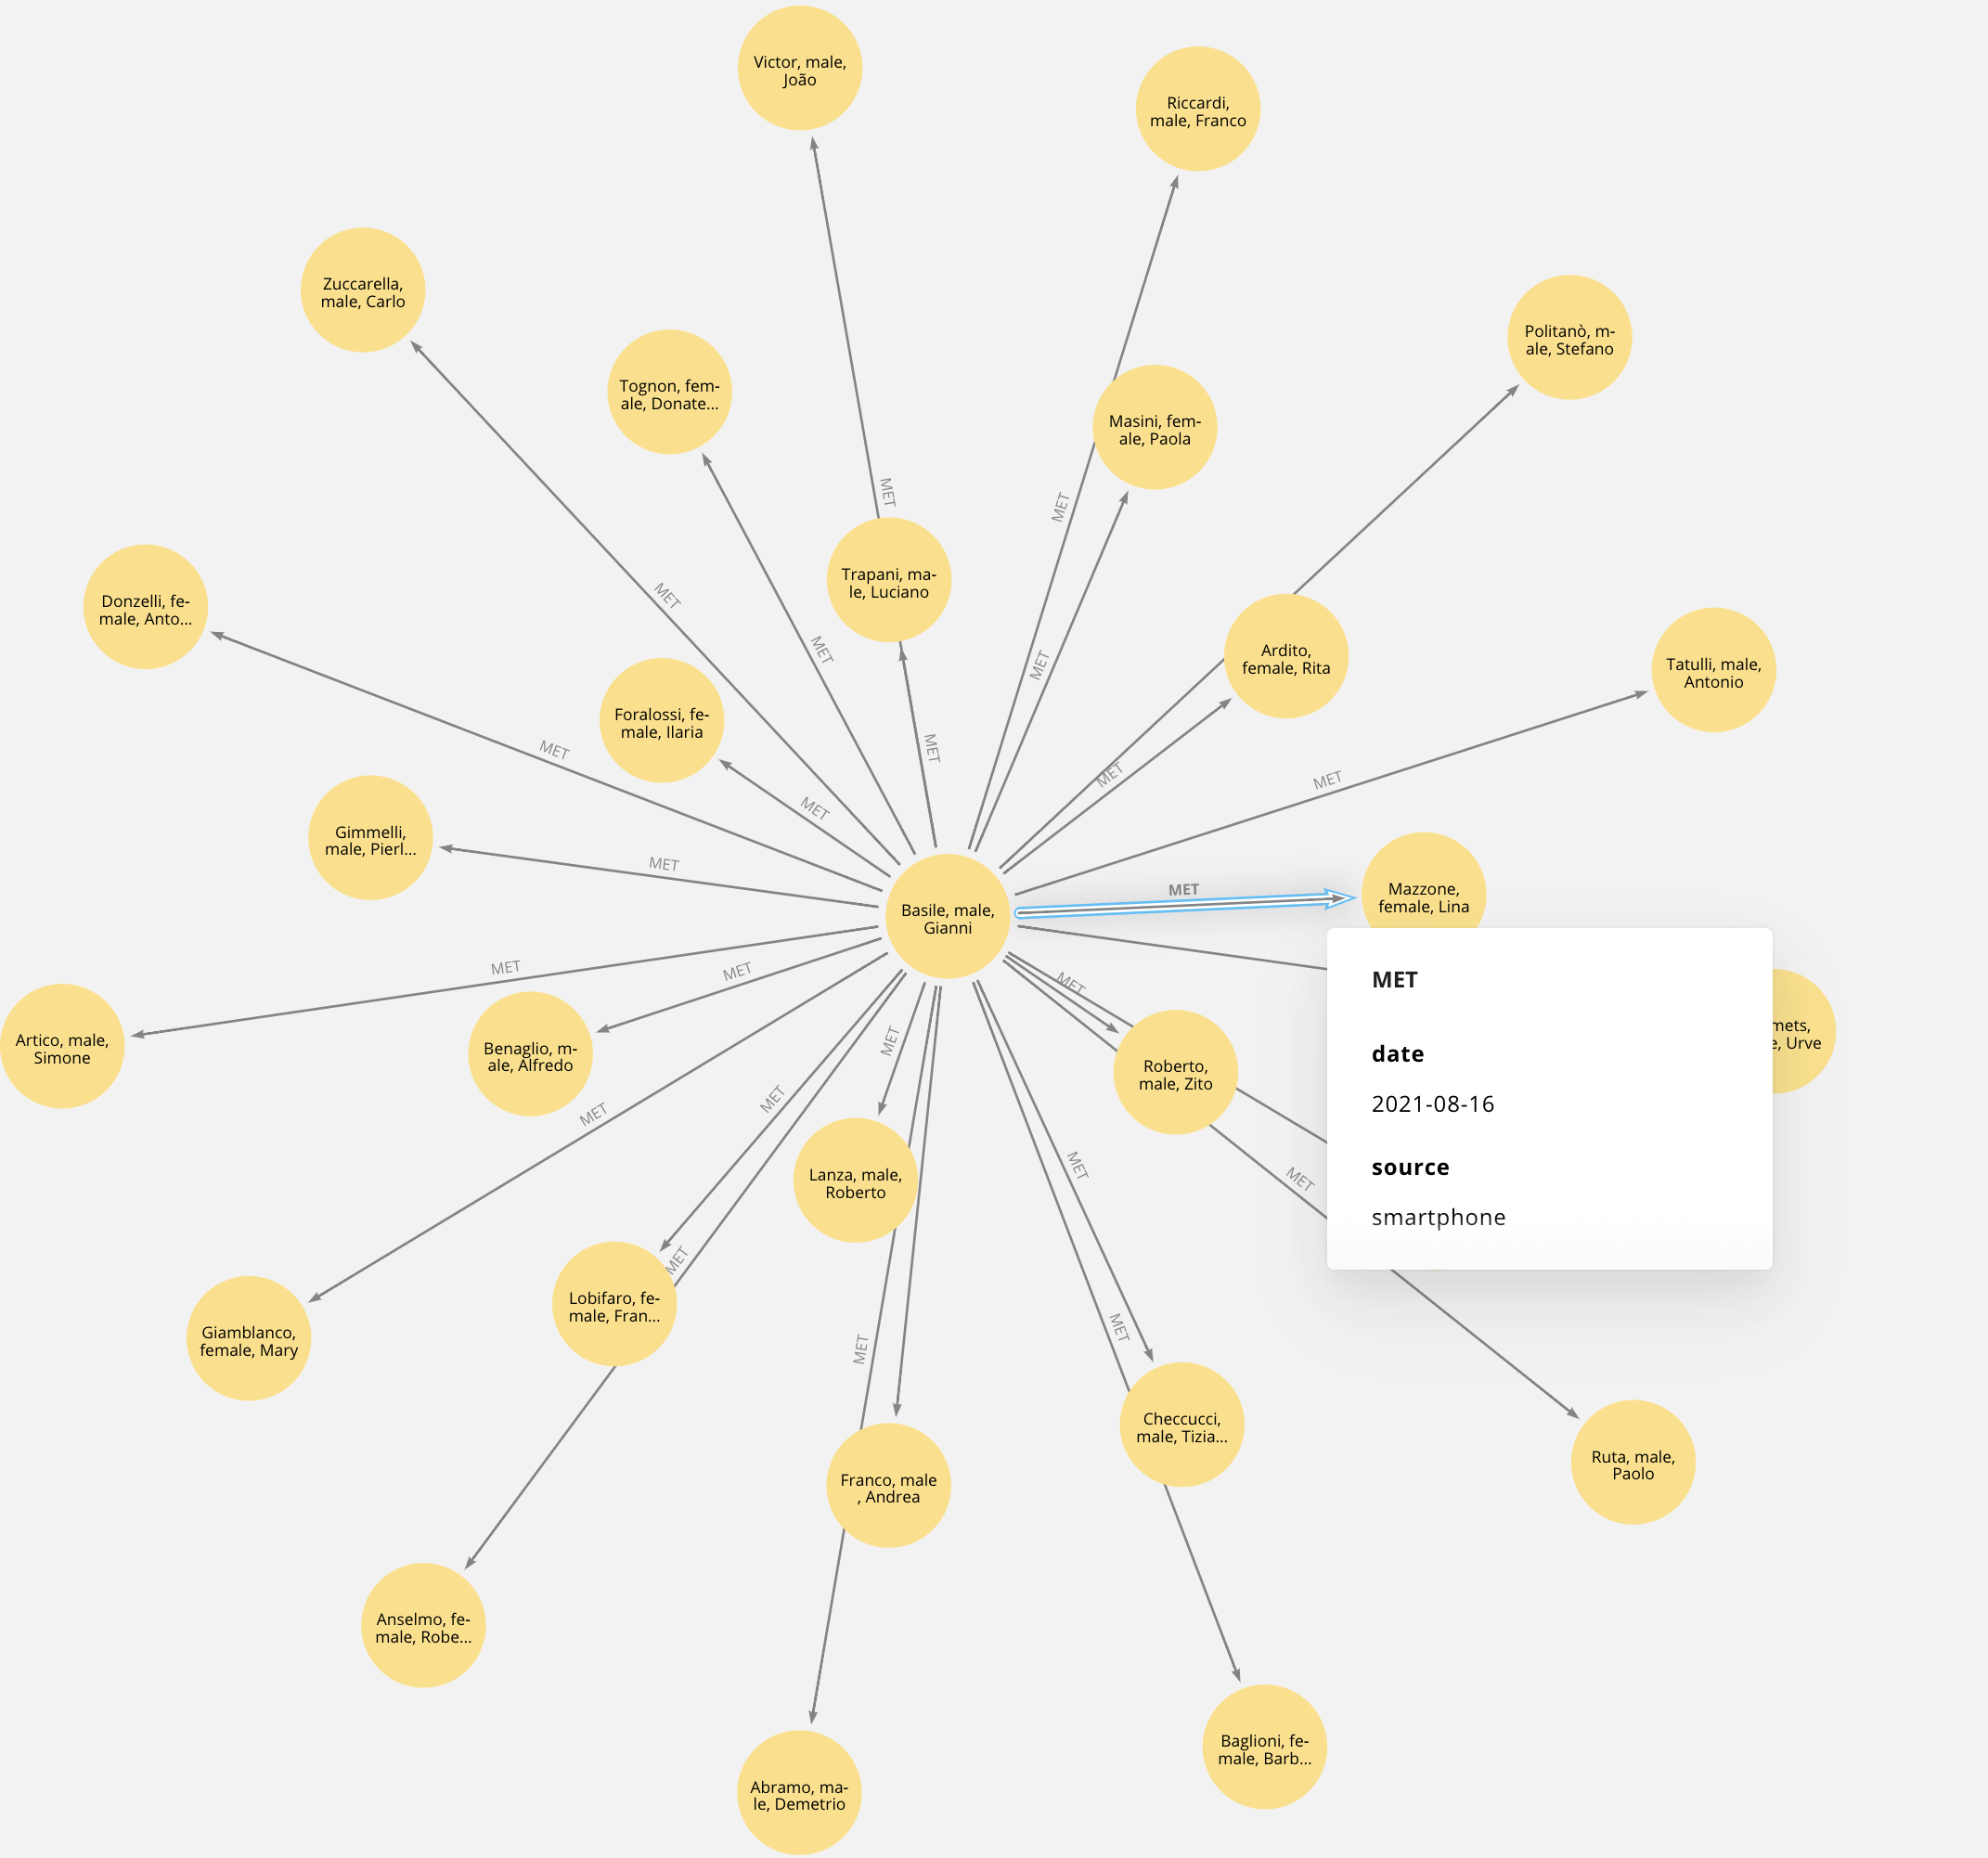
\includegraphics[width=0.7\linewidth, frame]{MET.png}
\caption{\emph{"MET"} Relationship Visualization}
\end{center}
\end{figure}


\subsubsection{LOCATED}

This directed relationship connects a \textbf{Place} node to a \textbf{City} node. We assume that each \textbf{Place} node is associated with exactly one \emph{"LOCATED"} relationship.
\\\\
The connection stores the following attributes: 
\begin{itemize}
    \item Address of the location
\end{itemize}

\begin{figure}[H]
\begin{center}
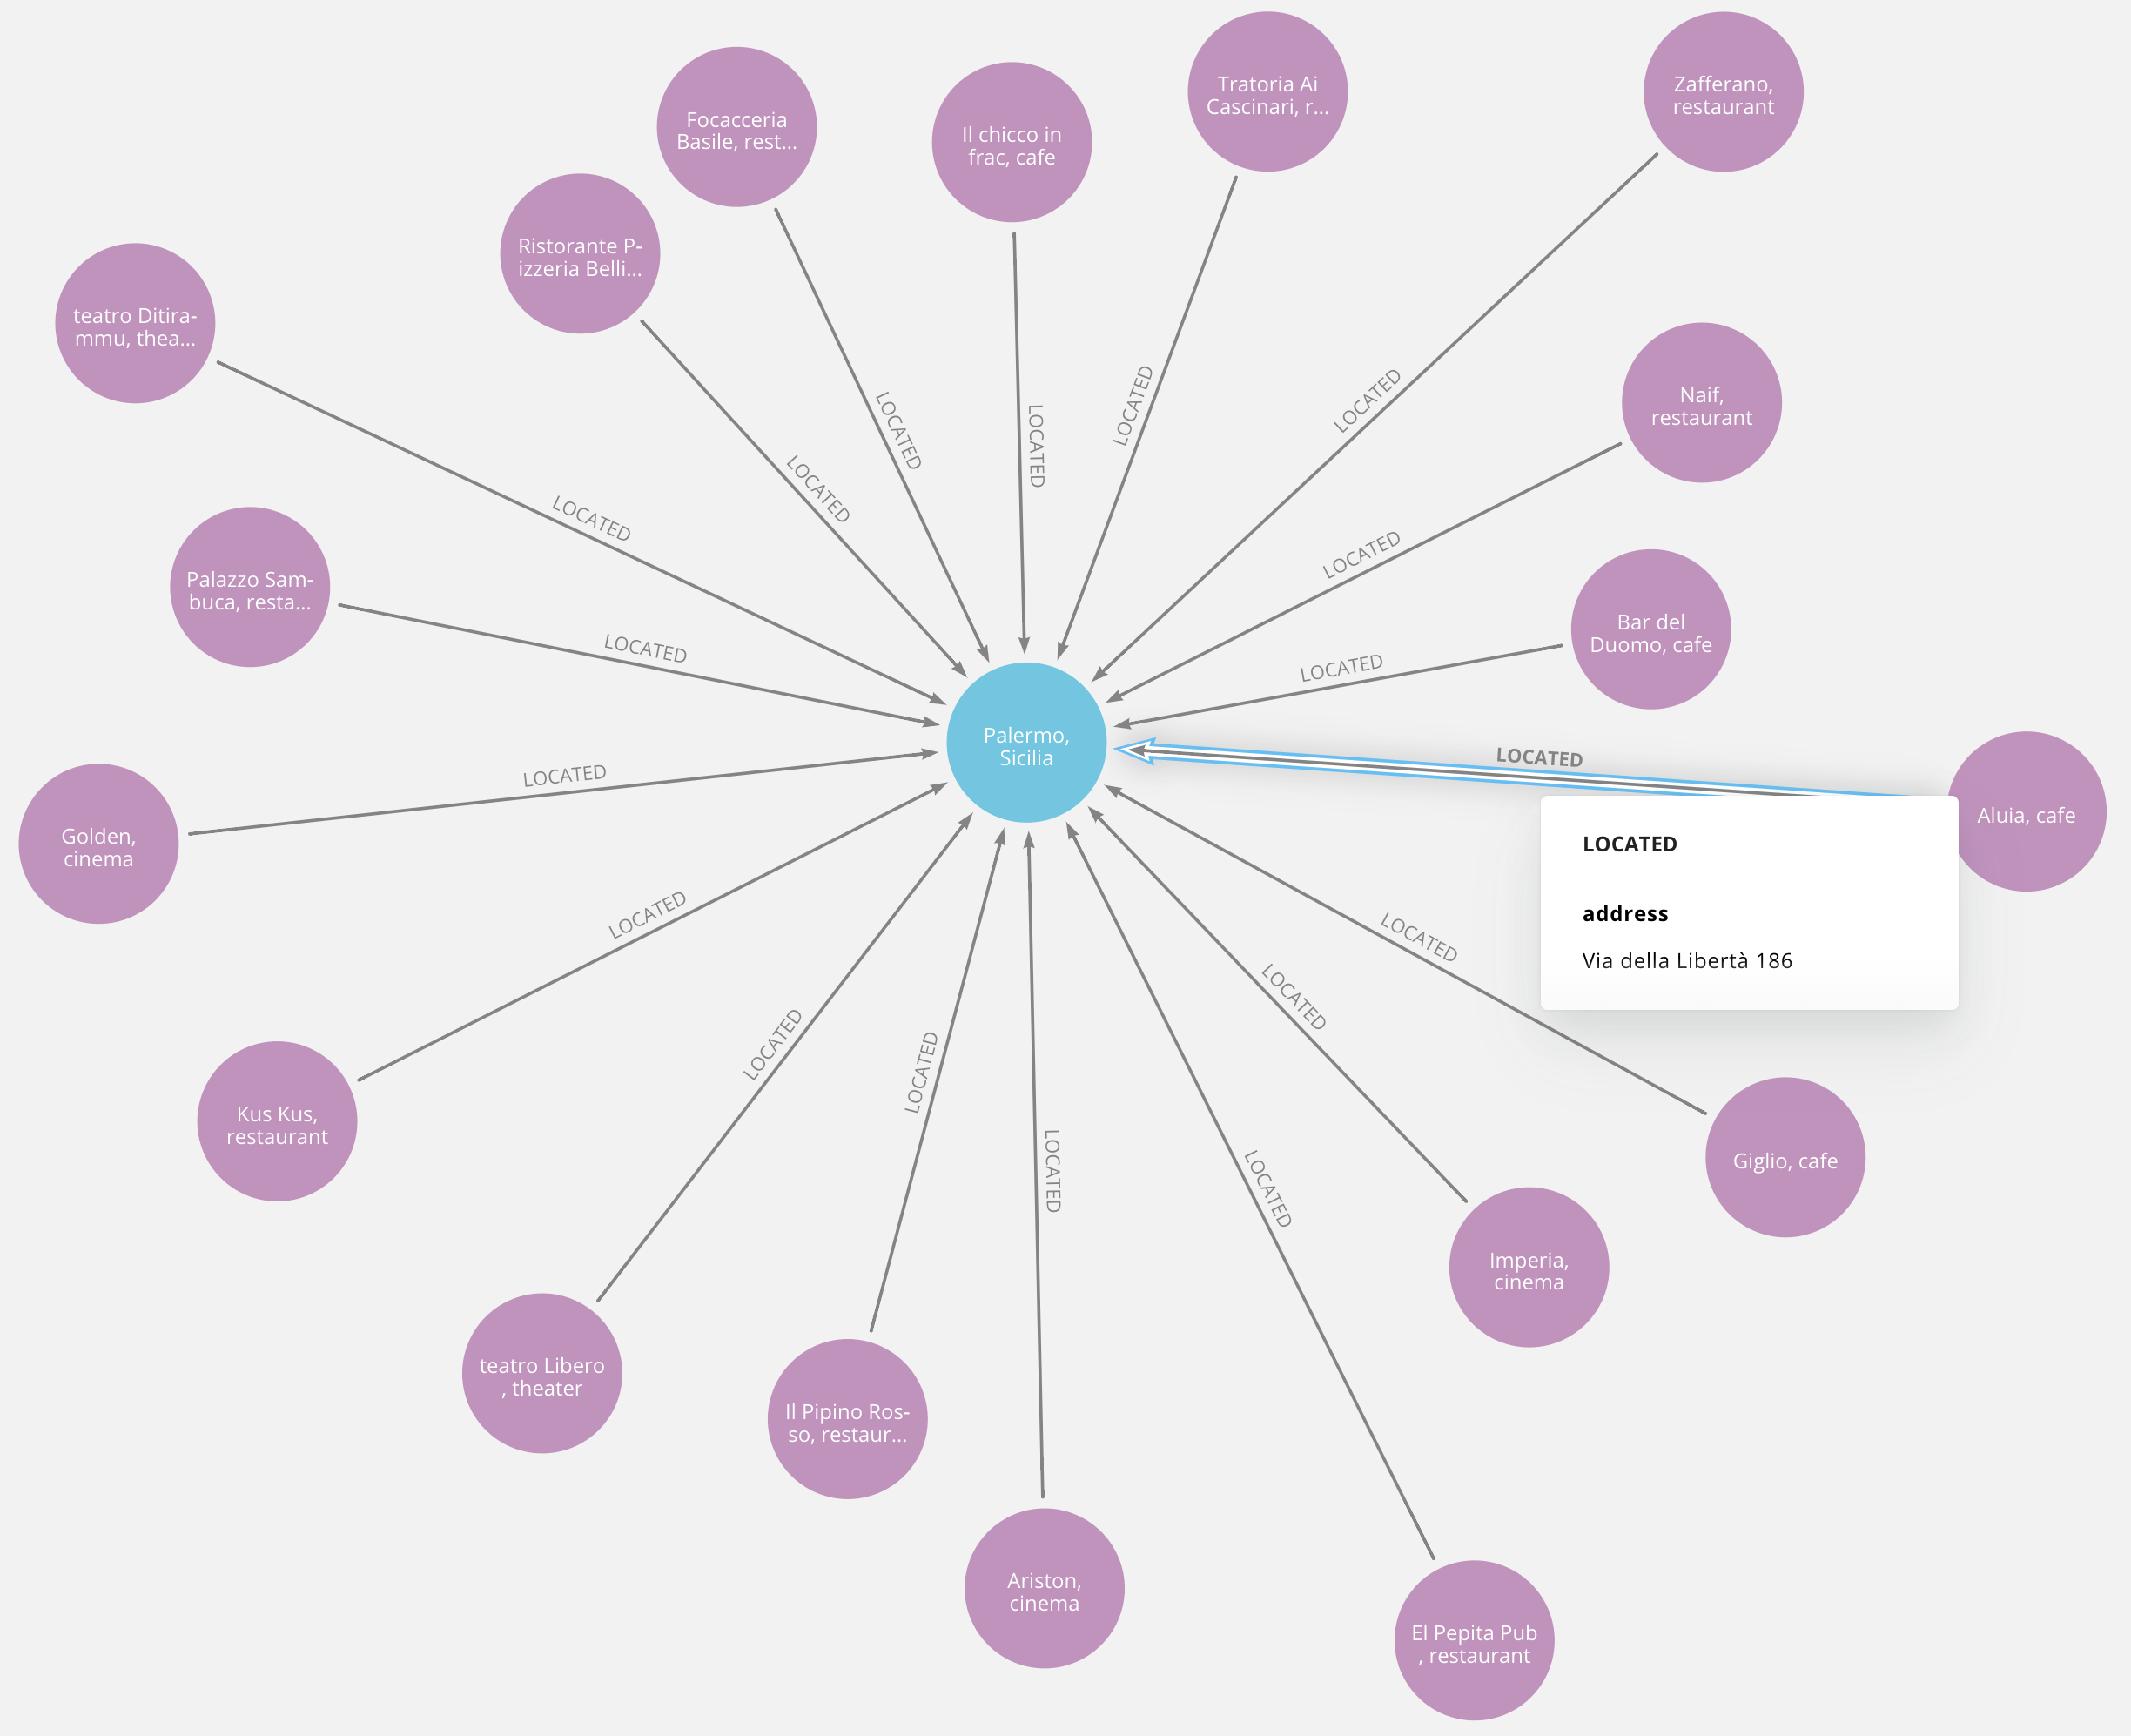
\includegraphics[width=0.65\textwidth, frame]{LOCATED.png}
\caption{\emph{"LOCATED"} Relationship Visualization}
\end{center}
\end{figure}


\subsubsection{PART OF}

This directed relationship connects a \textbf{City} node to a \textbf{State} node. We assume that each \textbf{City} node is associated with exactly one \emph{"PART OF"} relationship. The connection doesn't store attributes.

\begin{figure}[H]
\begin{center}
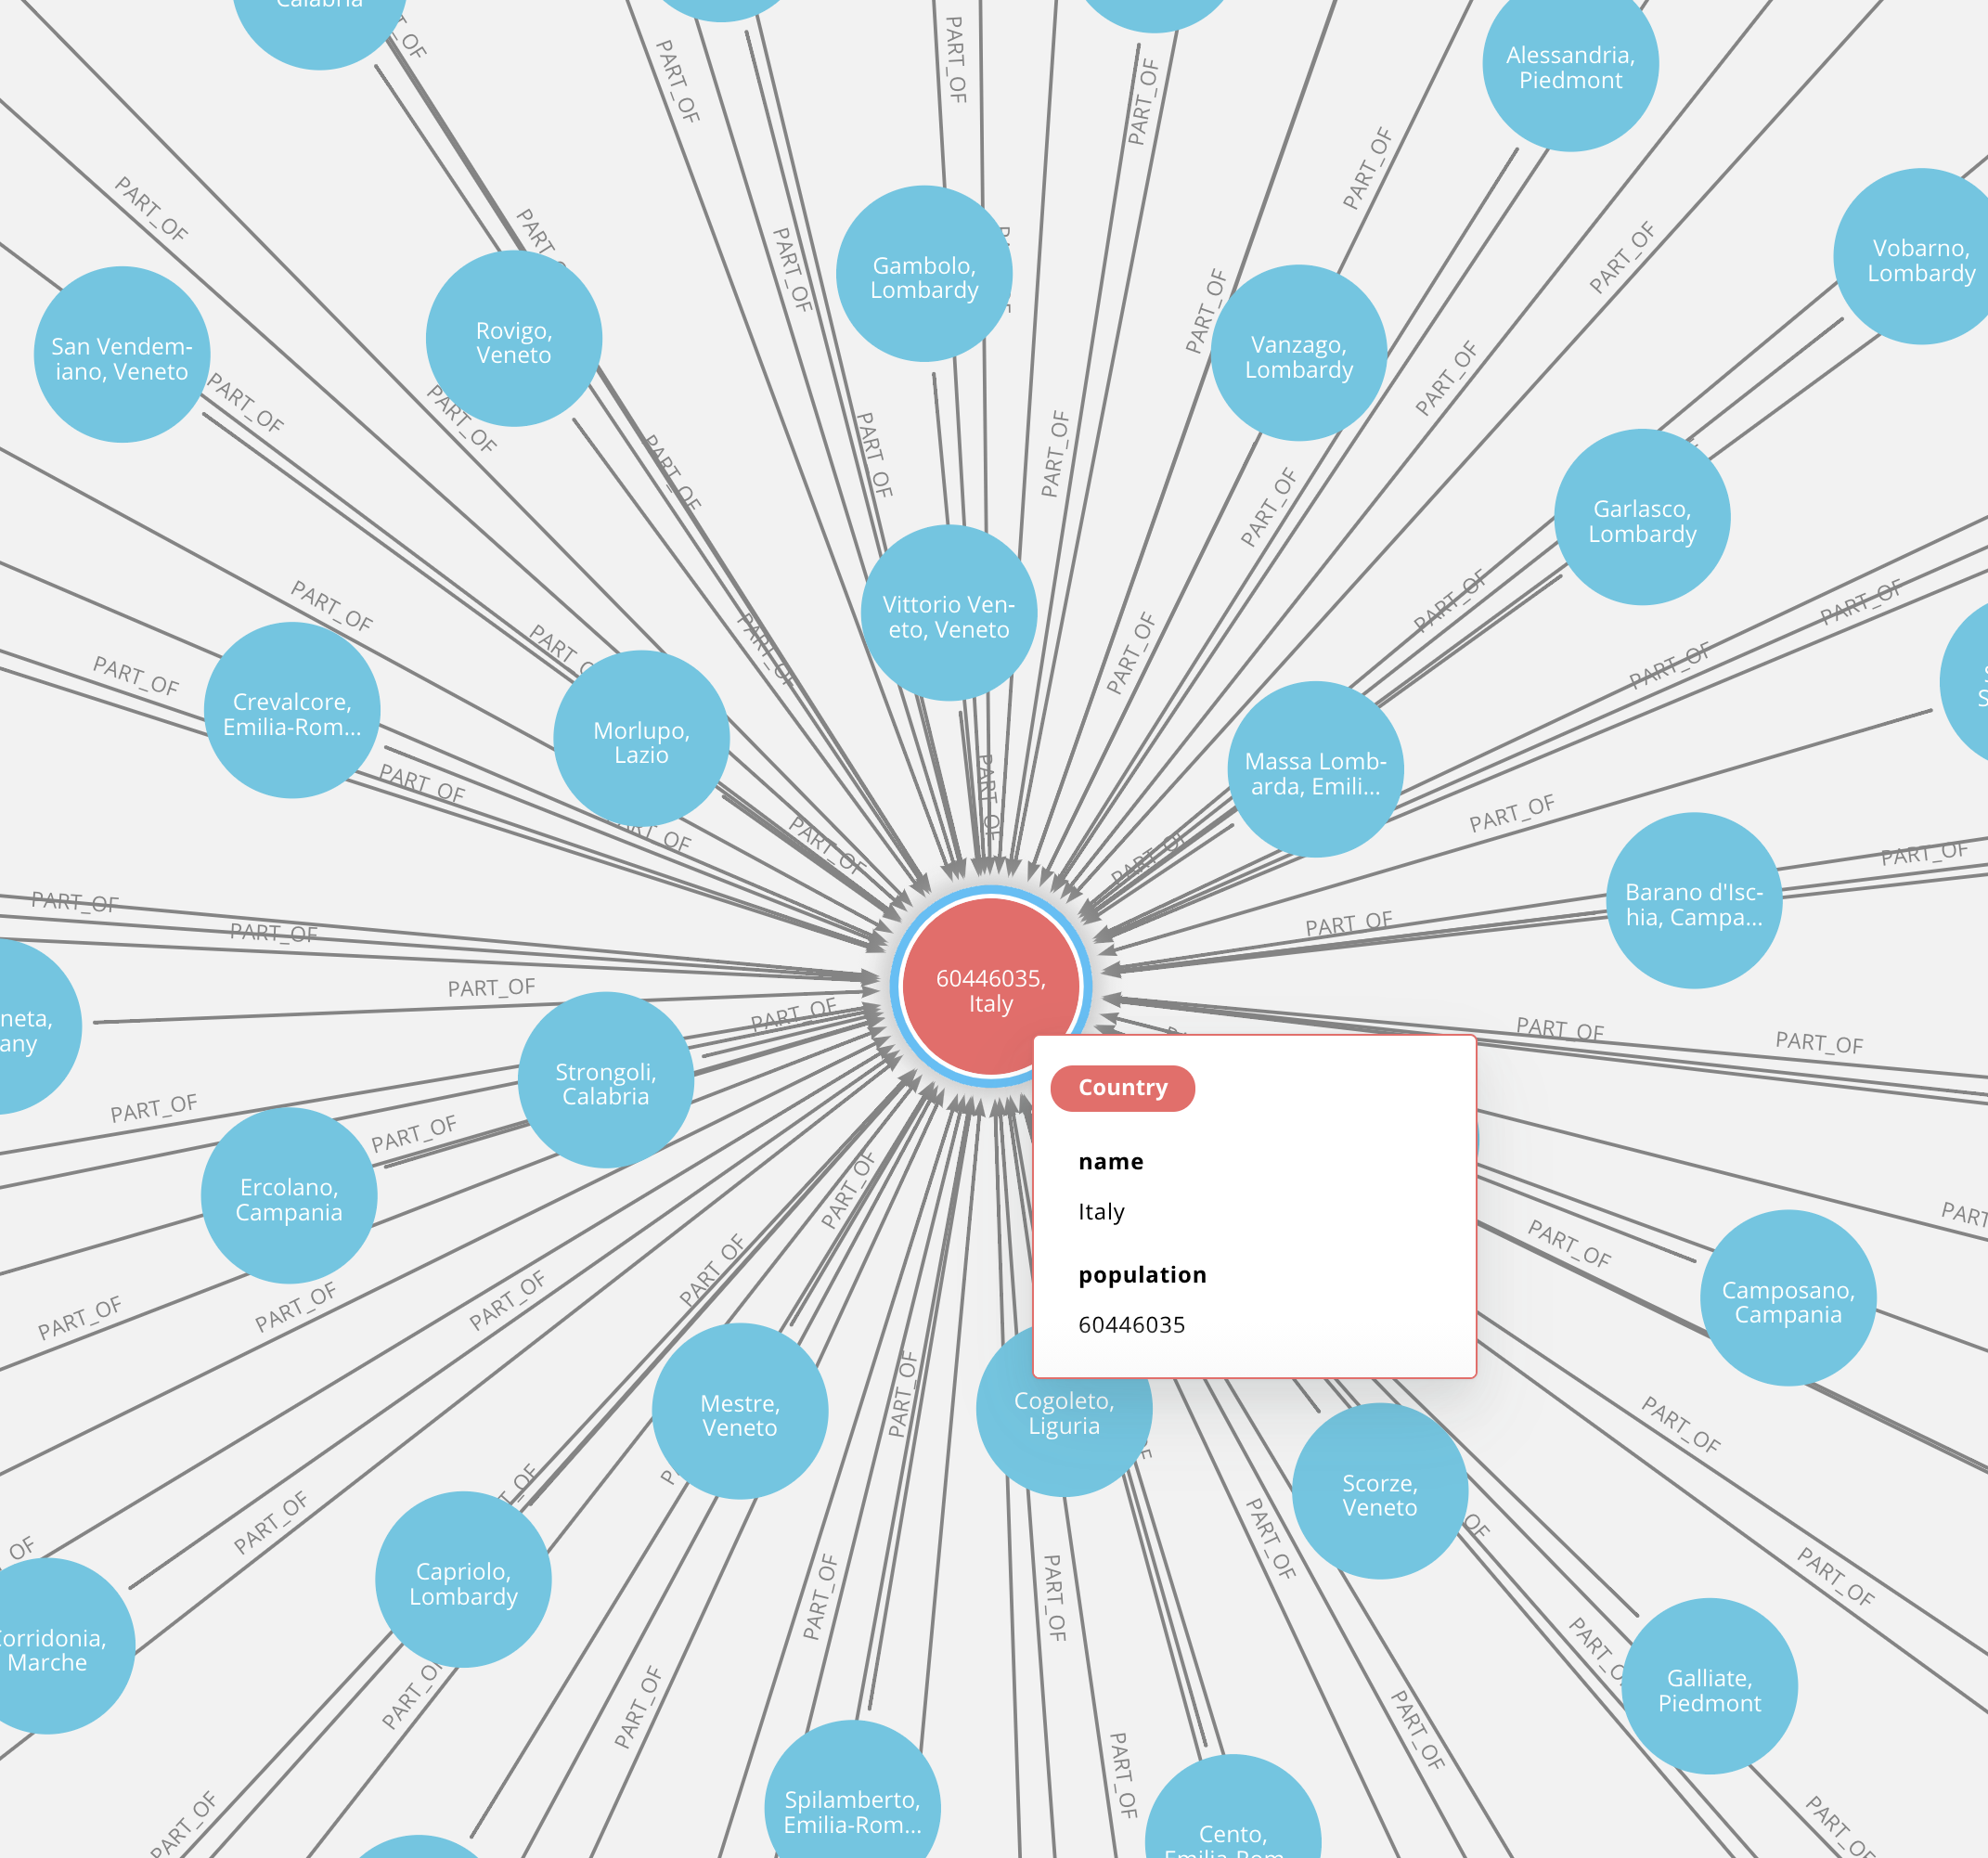
\includegraphics[width=0.65\linewidth, frame]{PART_OF.png}
\caption{\emph{"PART OF"} Relationship Visualization}
\end{center}
\end{figure}



\section{Database Creation}\label{db}
The database creation process has relied on various \textbf{CSV} datasets freely available online and on \textbf{Python}\cite{van1995python} programming language, in order to extract the information suitable to build an appropriate dataset \\ fulfilling our needs. Since information comes from different providers, such as public companies \\ (e.g \textbf{DatiOpen.it}), the need to have a data processing pipeline was high.
Thus through several Python functions and libraries we sequentially applied different modification to data, including:

\begin{itemize}
    \item Null fields rows removal
    \item Duplicate rows removal
    \item Standardization of fields to have only first letter uppercase
    \item Document delimiter conversion to match CSV standard (e.g from "\textbf{;}" to "\textbf{,}" delimiter)
    \item Generation of random documents IDs, with respect to the real document number format \\ (e.g : 2 letters and 7 digits for Italian passport number)
    \item  Address of places with \textbf{OpenStreetMap API}\cite{OpenStreetMap} or pick a random one if not found with given parameters
    \item Generation of random birth dates and assignment of random residence address, Covid tests, vaccine doses, visited places and contact tracking records to people.
\end{itemize}

In the following sections, along with a brief description of particular problems we had to face, for each entity of the database we show portions of initial and final structure of the corresponding CSV files.

\subsection{People}

The original data comes from the \textbf{2019 Facebook breach}\cite{facebookleak}. We selected a single text file coming from the Italian section of the dump, firstly reduced the amount of information (original file size is around \textbf{800 MB}) to 5000 entries, then we parsed it, dealing with a non standard data record format, removed unused information (such as relationship status) and added random realistic information (such as birth date).

\begin{figure}[H]
\begin{center}
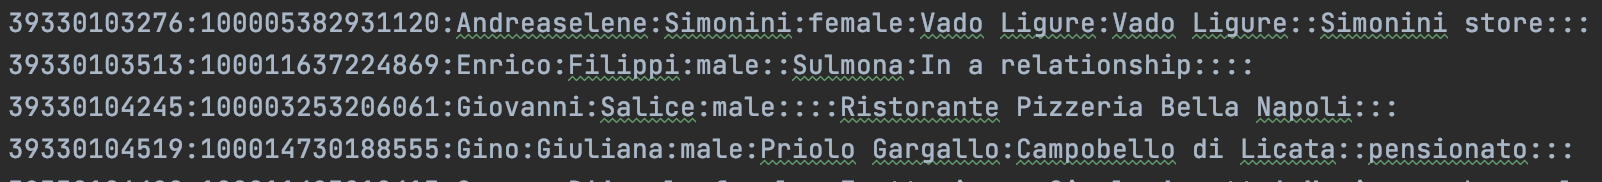
\includegraphics[width=0.5\linewidth, frame]{people_original.png}
\caption{Original structure}
\end{center}
\end{figure}


\begin{figure}[H]
\begin{center}
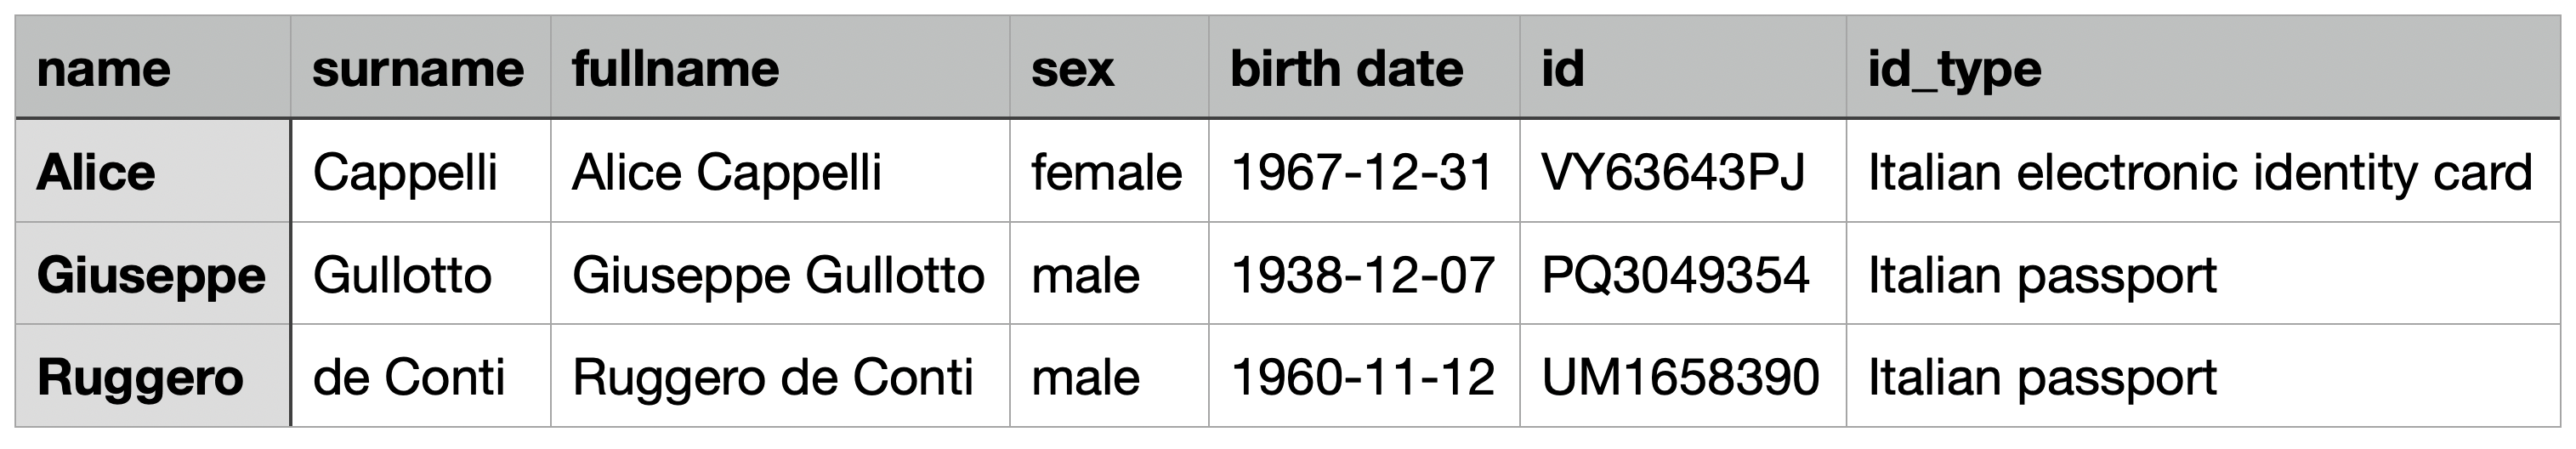
\includegraphics[width=0.5\linewidth, frame]{people.png}
\caption{Final structure}
\end{center}
\end{figure}


\subsection{Countries}

The original data come from a \textbf{Kaggle user}\cite{worldcountries}, from whose data we removed the median age lifespan field. 

 \begin{figure}[H]
    \centering
    \begin{minipage}{0.30\textwidth}
        \centering
        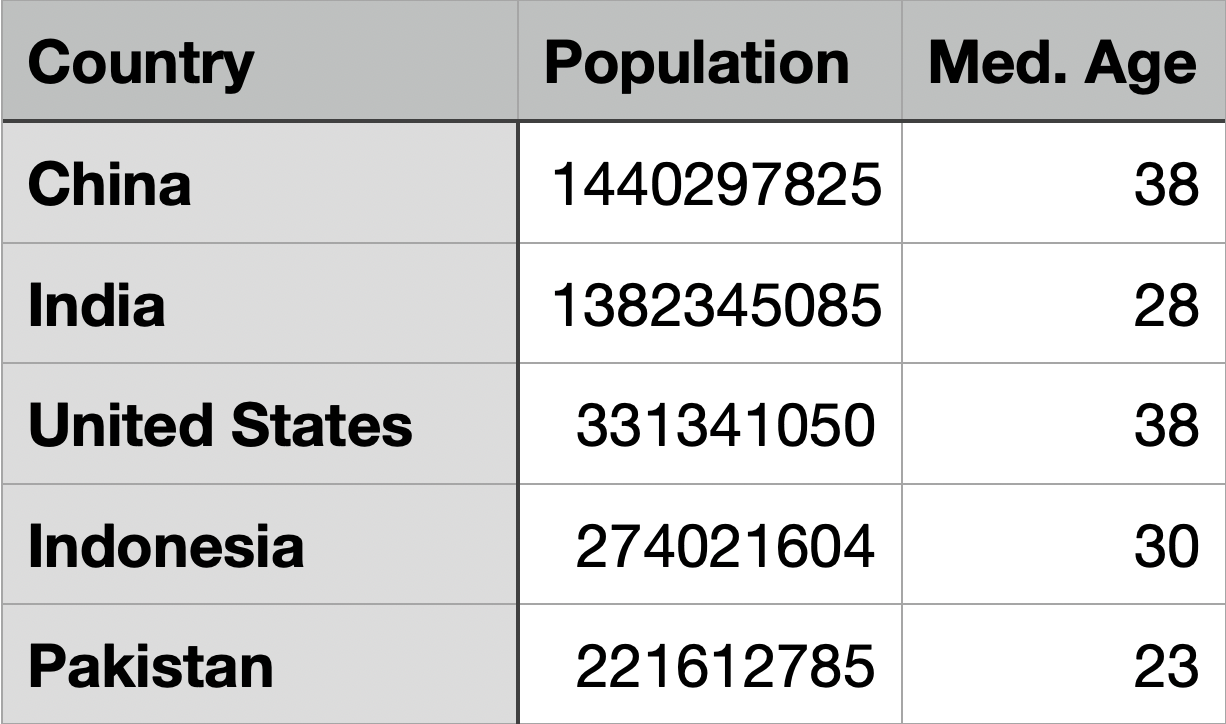
\includegraphics[width=1.1\textwidth,frame]{countries_original.png}
        \caption{Original structure}
    \end{minipage}
    \hspace{1cm}
    \begin{minipage}{0.30\textwidth}
        \centering
        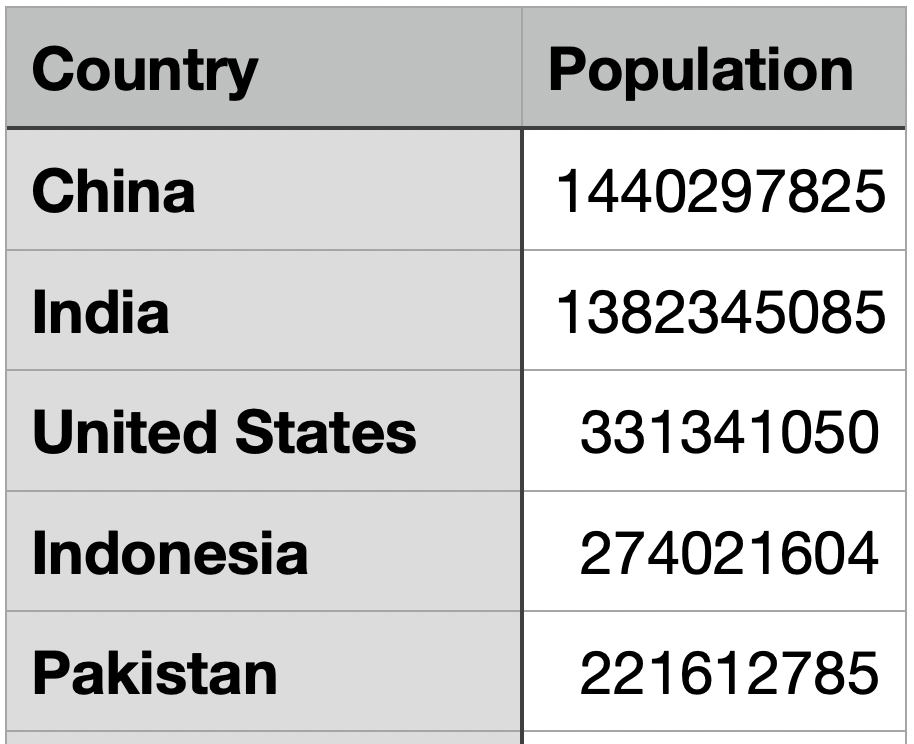
\includegraphics[width=0.8\textwidth, frame]{countries.png} 
        \caption{Final structure}
    \end{minipage}

\end{figure}



\subsection{Cities}

The original data comes from the \textbf{simplemaps}\cite{simplemaps} world cities csv dataset, from which we removed unused fields (such as \textbf{iso2} country code) and filtered out non Italian cities.  

\begin{figure}[H]
\begin{center}
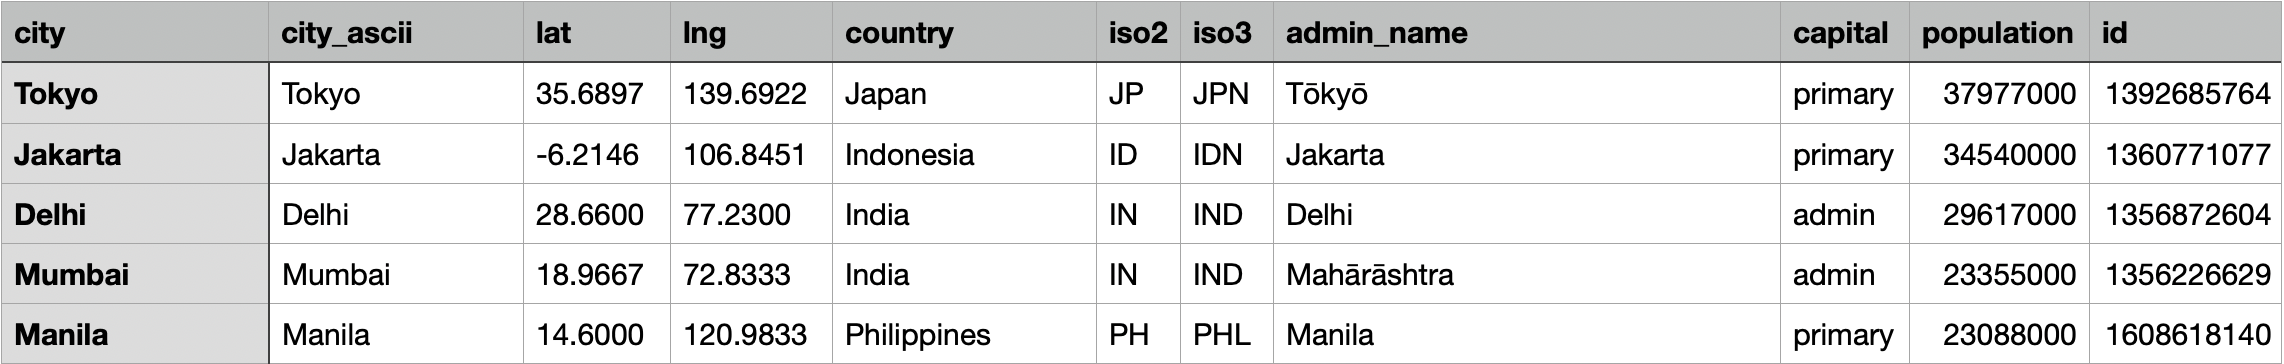
\includegraphics[width=0.5\linewidth, frame]{cities-w_original.png}
\caption{Original structure}
\end{center}
\end{figure}

\begin{figure}[H]
\begin{center}
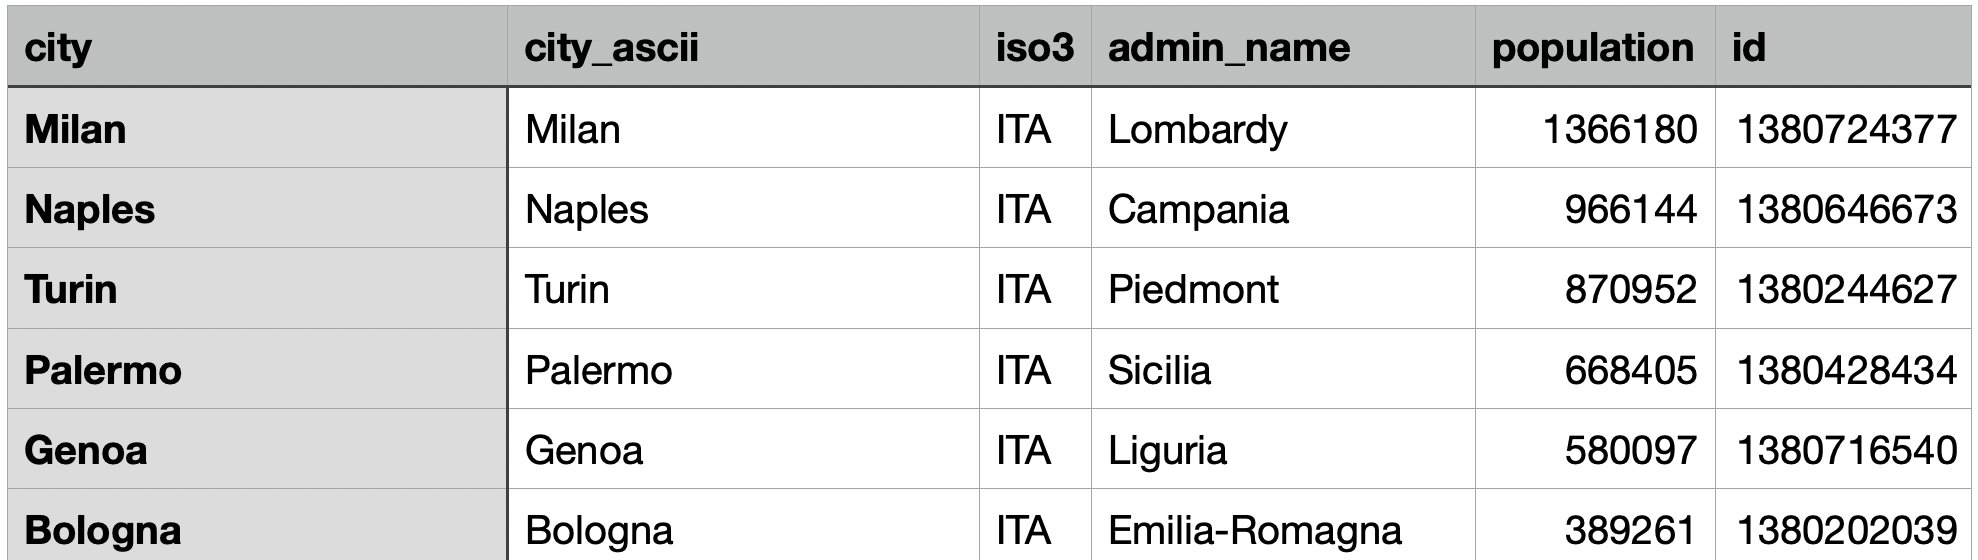
\includegraphics[width=0.5\linewidth, frame]{cities.png}
\caption{Final structure}
\end{center}
\end{figure}


\subsection{Places}

Since we decided to focus on an Italian oriented dataset, original CSVs were retrieved from the Italian Open Data website \textbf{DatiOpen.it}\cite{datiopen}. Although we were able to find datasets about restaurants, cafes, theaters, cinemas and hospitals, the separator in all these files is a semicolon, a lot of data is duplicated or missing and an \textbf{OpenStreetMap ID} is used instead of an explicit address. Even though this ID is used in our database, to have meaningful entries we needed to retrieve, when possible, through the \textbf{OpenStreetMap API}, or pick randomly, a huge amount of addresses, since some of these files have more than \textbf{30.000} records.



\begin{figure}[H]
\begin{center}
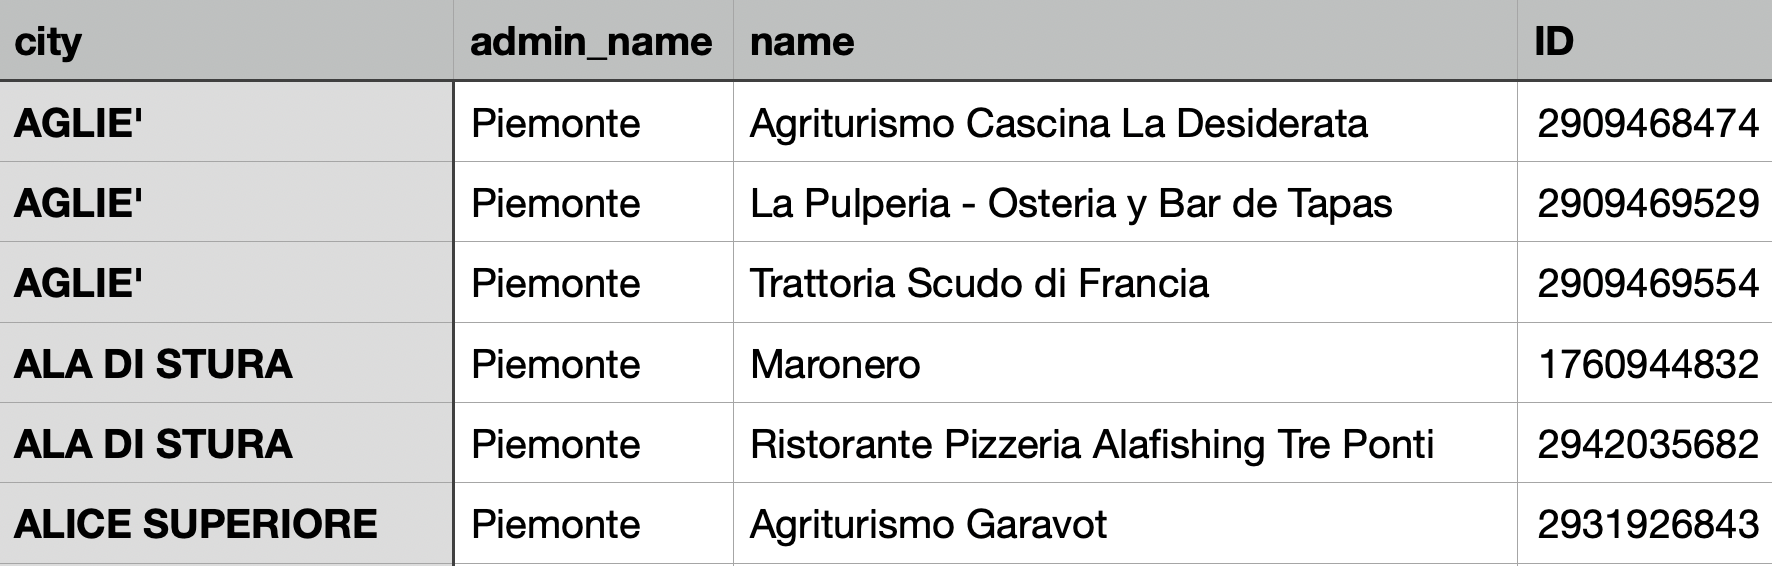
\includegraphics[width=0.5\linewidth, frame]{restaurants_original.png}
\caption{Original structure}
\end{center}
\end{figure}

\begin{figure}[H]
\begin{center}
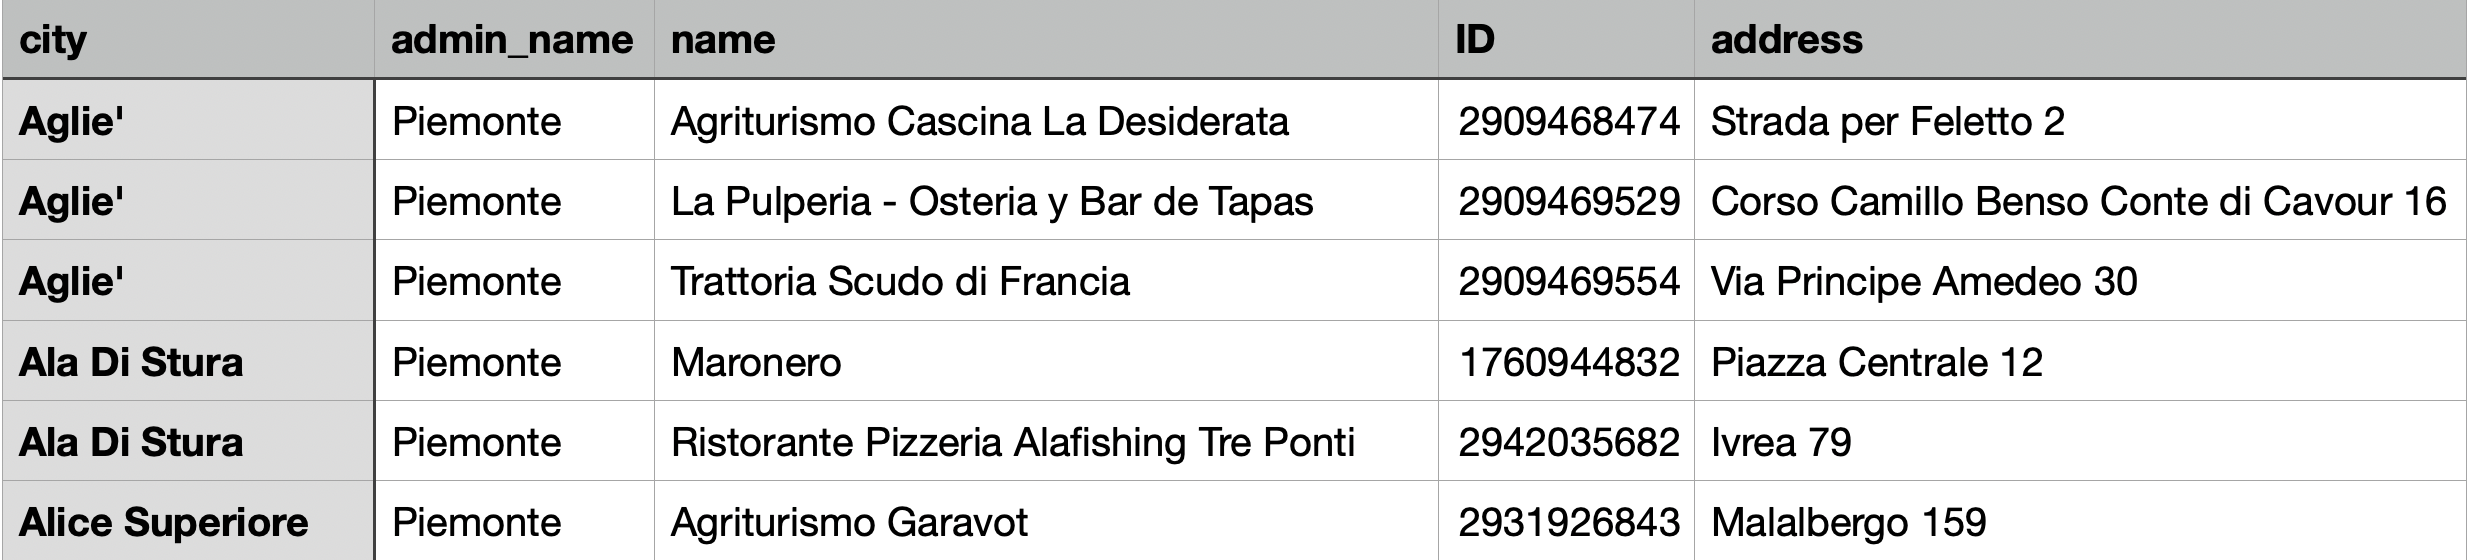
\includegraphics[width=0.5\linewidth, frame]{restaurants.png}
\caption{Final structure}
\end{center}
\end{figure}

\newpage

\subsection{Tests \& Vaccines}

The Vaccines CSV containing information related to world countries comes from \textbf{ourworldindata.org} \cite{ourworldindata} and didn't need manipulations. The covid test type CSV was written from scratch with reference to a \textbf{FDA article} \cite{fdatesting} regarding Covid tests.

 \begin{figure}[H]
    \centering
    \begin{minipage}{0.30\textwidth}
        \centering
        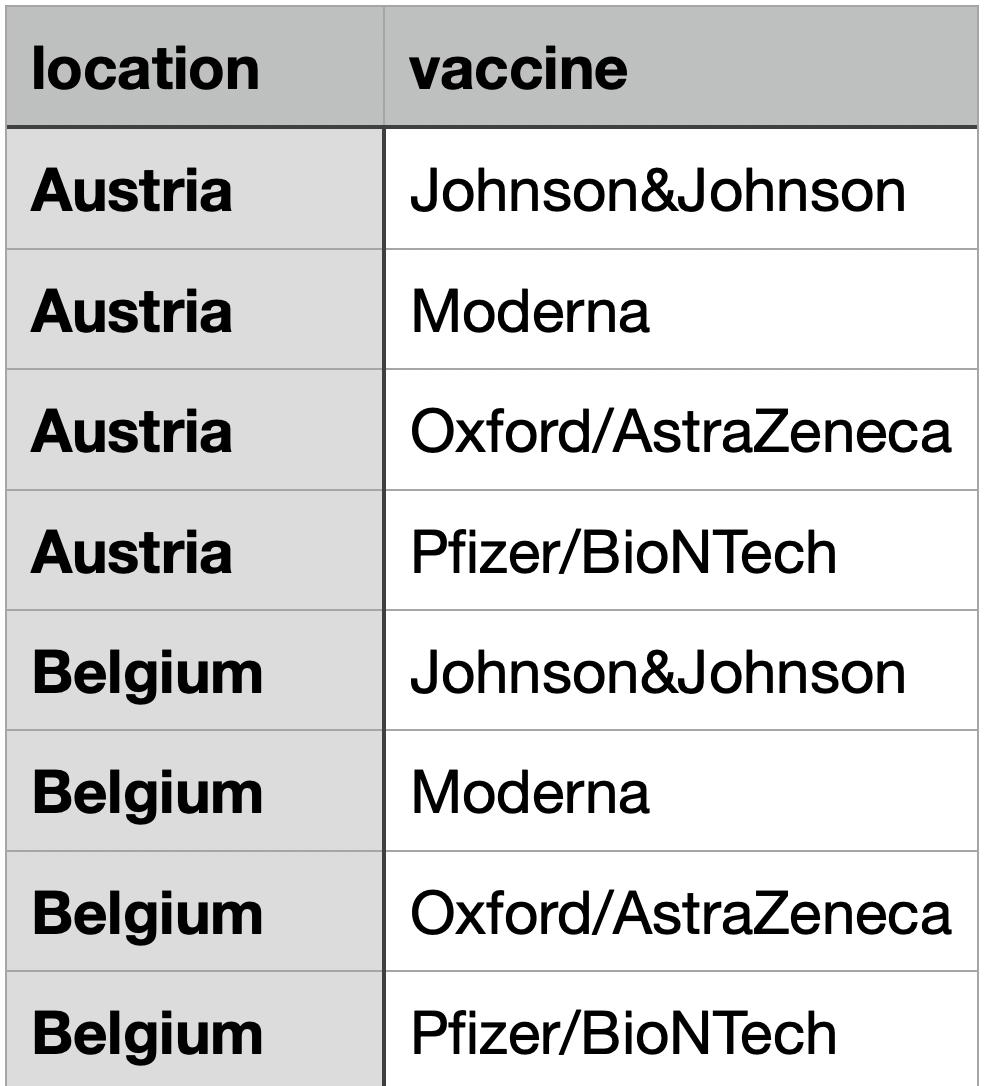
\includegraphics[width=0.8\textwidth,frame]{vaccines_by_country.png}
    \end{minipage}
    \begin{minipage}{0.30\textwidth}\hfill
        \centering
        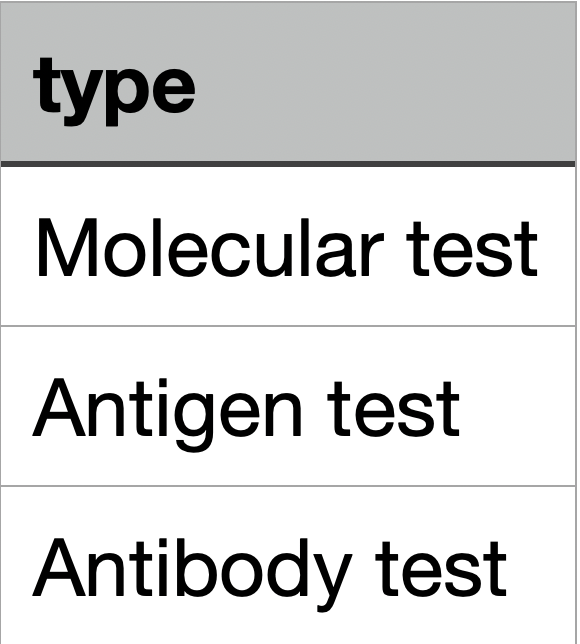
\includegraphics[width=0.8\textwidth, frame]{covid_test.png} 
    \end{minipage}
    \caption{Final structures}
\end{figure}

\subsection{Relationships}
In this subsection some of the relationships are briefly described from a creation point of view, highlighting the random data generation procedures handled to create pseudo realistic database content:

\begin{itemize}

    \item \textbf{RECEIVED}: 25\% of people have a single dose of Vaccine, whose administration ranges from \textbf{2021-10-7} to \textbf{2021-11-7}. Moreover 25\% of people have a double dose of Vaccine, whose first dose ranges from \textbf{2021-01-05} to \textbf{2021-06-05} and the second dose's date is \textbf{after 28 days}. In both cases assignment of vaccination dates has been done starting from the eldest.
    
    \item \textbf{TOOK}: each person has a randomly picked number of samples assigned, whose date ranges from \textbf{2021-01-05} to \textbf{2021-11-7} and whose outcome is determined randomly.
    
    \item \textbf{WENT TO}: each person is associated with \textbf{50} places in the database through this relationship. Places are picked randomly and retrieved through their unique ID, moreover the registration date ranges from \textbf{2020-3-10} to \textbf{2021-11-07}.
    
    \item \textbf{LIVES WITH}: this relationship is created forming randomly groups of cohabitants sizing from 1 to 6 people. 
    
    \item \textbf{LIVES IN}: this relationship's creation is strictly related to the previous one, since the same randomly picked address is assigned to each cohabitant.
    
    \item \textbf{MET}: this is the most time consuming relationship creation among the ones involved in database creation. A random amount of \textbf{MET} relationships, ranging form 10 to 50, is assigned to each person. For each creation
    various steps are performed. Firstly a random place ID is picked. Then a random person ID is picked, with appropriate checks to avoid reflexive relationships. Lastly a query is performed to verify that the two people aren't living together, if so the relationship is created, with a date attribute ranging from \textbf{2020-03-10} to \textbf{2021-11-07}.
    
\end{itemize}


\newpage

\section{Queries \& Commands}\label{cmd-que}

\subsection{Queries}

The following subsection presents some useful queries and their possible textual result, with the aim of showing database's utility

\begin{itemize}

    \item Find the Country with the highest number of positive Covid samples taken
    
    \begin{lstlisting}
    
    MATCH (:Test)-[took:TOOK]-(p:Person)-[:LIVES_IN]-(c:City)-[:PART_OF]-(s:Country)
    WHERE took.isPositive = true
    WITH COUNT(p) AS positive_samples, s.name AS country
    ORDER BY positive_samples DESC
    LIMIT 1
    RETURN country, positive_samples
    \end{lstlisting}
    
    \vspace{-0.5cm}
    
    \begin{table}[H]
    \hspace{1.55cm}
    \begin{tabular}{|l|l|}
    \hline
    \textbf{country} & \textbf{positive\_samples} \\ \hline
    Italy            & 10763                    \\ \hline
    \end{tabular}
    \end{table}
    
    \item Find the place where the highest number of people, tested positive to a Covid sample performed on a certain date, went in the previous n (e.g. 300) days.
    
    \begin{lstlisting}
    
    MATCH (:Test)-[took:TOOK]-(p:Person)-[w:WENT_TO]-(place:Place)-
    [l:LOCATED]-(c:City)-[pa:PART_OF]-(co:Country)
    WHERE took.isPositive = true
    AND took.date = date('2021-1-1')
    AND w.date >= took.date - duration({days: 300})
    AND w.date <= took.date
    WITH COUNT(p) AS people, place.name AS name, place.type AS type,
    l.address + ", " + c.name + ", " + c.region + ", " + co.name AS address
    ORDER BY people DESC
    LIMIT 1
    RETURN name, type, address, people;

    
    \end{lstlisting}
    
    \vspace{-1.1cm}
    
    \begin{table}[H]
    \hspace{1.48cm}
    \begin{tabular}{|c|c|c|c|}
    \hline
    \textbf{name}    & \textbf{type} & \textbf{address}                            & \textbf{people} \\ \hline
    ABCinema d'Essai & cinema        & Vicolo Baratono 124, Ivrea, Piedmont, Italy & 63784               \\ \hline
    \end{tabular}
    \end{table}
    
    \item List of people who tested positive to a Covid sample and the count of people they met over the last n (e.g.: 300) days
    
    \begin{lstlisting}
    
    MATCH (t:Test)-[took:TOOK]-(p1:Person)-[m:MET]->(p2:Person)
    WHERE took.isPositive = true 
    AND m.date >= took.date - duration({days: 300})  
    AND m.date <= took.date
    WITH COUNT(p2) AS people_met, p1.name AS name
    ORDER BY people_met DESC
    RETURN name, people_met;

    \end{lstlisting}
    
    \vspace{-1cm}
        
        
    \begin{table}[h]
    \hspace{1.48cm}
    \begin{tabular}{|c|c|}
    \hline
    \textbf{name}     & \textbf{people\_met} \\ \hline
    Carlo Solinas     & 1494                 \\ \hline
    Franco Lai        & 1194                 \\ \hline
    Giannino Molinaro & 1186                 \\ \hline
    Mario Facchini    & 1178                 \\ \hline
    Nico Borracci     & 1177                 \\ \hline
    \end{tabular}
    \end{table}
    
    \newpage
        
    \item Find the city with the highest number of first dose vaccinated people up to a given date
    
    \begin{lstlisting}
    
    MATCH (:Vaccine)-[r:RECEIVED]-(p:Person)-[:LIVES_IN]-(c:City)-[:PART_OF]-(co:Country)
    WHERE r.date <= date('2022-01-01') 
    AND r.number = 1
    WITH COUNT(p) AS people, 
    c.name + ", " + c.region + ", " + co.name AS city
    ORDER BY people DESC
    LIMIT 1
    RETURN city, people;

    \end{lstlisting}
    
    \vspace{-1cm}
    
    \begin{table}[h]
    \hspace{1.48cm}
    \begin{tabular}{|c|c|}
    \hline
    \textbf{city}            & \textbf{people} \\ \hline
    Milano, Lombardia, Italy & 1076041         \\ \hline
    \end{tabular}%
    \end{table}
    
    \item Find the tracking source that registered the highest number of contacts
    
    \begin{lstlisting}
    
    MATCH ()-[m:MET]->()
    WITH m.source AS source, COUNT(m.source) AS num_sources
    ORDER BY num_sources DESC
    LIMIT 1
    RETURN source, num_sources;

    \end{lstlisting}
    
    \vspace{-1cm}
    
    \begin{table}[H]
    \hspace{1.48cm}
    \begin{tabular}{|l|l|}
    \hline
    \textbf{source} & \textbf{num\_contacts} \\ \hline
    \multicolumn{1}{|c|}{smartphone}      & \multicolumn{1}{|c|}{27634} \\ \hline
    \end{tabular}
    \end{table}
    
    \item Find the age range (\textbf{10 years}) who has been infected the most and the number of
    infections \\ (in relation to the number of people composing that category)

    \begin{lstlisting}
    
    MATCH (:Test)-[took:TOOK]-(p:Person)
    WITH "["+(duration.between(p.birthDate,datetime()).years/10)*10+","
    +(duration.between(p.birthDate,datetime()).years/10+1)*10+")" AS age_range,
    COUNT(*) AS total_people, 
    SUM(CASE WHEN took.isPositive = true THEN 1 ELSE 0 END) AS positive_people,
    SUM(CASE WHEN took.isPositive = true THEN 1 ELSE 0 END)*1.0/COUNT(*) AS rate
    ORDER BY rate DESC
    LIMIT 1
    RETURN age_range,total_people,positive_people, round(rate, 2, 'HALF_UP');

    \end{lstlisting}
    
    \vspace{-1cm}
    
    \begin{table}[H]
    \hspace{1.48cm}
    \begin{tabular}{|c|c|c|c|}
    \hline
    \textbf{age\_range} & \textbf{total\_people} & \textbf{positive\_people} & \textbf{rate}     \\ \hline
    {[}10,20)           & 8543                   & 4676                      & 0.55 \\ \hline
    \end{tabular}%
    \end{table}
    
    \item  Find the vaccine with less positive samples registered until a certain date \\ (in relation to the number of days past the vaccination)
    
    \begin{lstlisting}
    
    MATCH (v:Vaccine)-[r:RECEIVED]-(p:Person)-[took:TOOK]-(test:Test)
    WHERE r.number = 1
    WITH v.manufacturer AS manufacturer, 
    SUM(CASE WHEN took.isPositive = true AND r.date <= took.date THEN 1 ELSE 0 END) 
    AS positive_people, 
    SUM(duration.inDays(r.date, date('2021-11-7')).days) AS total_days
    ORDER BY total_days/positive_people ASC
    RETURN manufacturer, total_days/positive_people;
    
    \end{lstlisting}
    
    \vspace{-0.5cm}
    
    \begin{table}[H]
    \hspace{1.48cm}
    \begin{tabular}{|c|c|}
    \hline
    \textbf{manufacturer} & \textbf{total\_days/positive\_people} \\ \hline
    Johnson\&Johnson      & 835                                   \\ \hline
    Pfizer/BioNTech       & 1262                                  \\ \hline
    Oxford/AstraZeneca    & 1321                                  \\ \hline
    Moderna               & 1372                                  \\ \hline
   
    \end{tabular}
    \end{table}
    
    \newpage
    
\item List the places visited by a given person over the last n (e.g.: 300) days 
starting from the positive Covid sample taken in a given date
    
    \begin{lstlisting}
    
    MATCH (:Test)-[took:TOOK]-(p:Person)-[w:WENT_TO]-(place:Place)-
    [l:LOCATED]-(city:City)-[pa:PART_OF]-(c:Country)
    WHERE p.fullname = 'Nanda Donati'
    AND took.isPositive = TRUE
    AND took.date = date('2020-07-29')
    AND w.date >= took.date - duration({days: 20})
    AND w.date <= took.date
    WITH place.name AS name, 
    l.address + ", " + city.name + ", " + city.region + ", " + c.name AS address,
    w.date AS date, place.type AS type
    ORDER BY date
    RETURN name, type, address, date;

    
    \end{lstlisting}
    
    \vspace{-1.2cm}

    \begin{table}[H]
    \hspace{-1cm}
    \begin{tabular}{|c|c|c|c|}
    \hline
    \textbf{name}             & \textbf{type} & \textbf{address}                                                 & \textbf{date} \\ \hline
    Movie Planet              & cinema        & Via della Libertà 84, Bellinzago Novarese, Piedmont, Italy       & "2020-12-14"  \\ \hline
    Ospedale dei villeggianti & hospital      & Ciclabile lungomare di Rimini 111, Rimini, Emilia-Romagna, Italy & "2020-12-22"  \\ \hline
    Antico Caffè Centrale     & cafe          & Via della Repubblica 38, Barga, Tuscany, Italy                   & "2020-12-27"  \\ \hline
    \end{tabular}
    \end{table}    

\end{itemize}

\subsection{Commands}

The following subsection presents some useful commands, with the aim of showing database’s utility.

\begin{itemize}
    \item \textbf{CSV LOAD Commands}. Column names are shown in paragraph 4.
    \begin{itemize}
        \item Person nodes CSV Load
        
        \begin{lstlisting}
        
        LOAD CSV WITH HEADERS FROM $path
        AS line FIELDTERMINATOR ','
        WITH line
        MERGE (:Person 
        {name: line.name, 
        surname: line.surname,
        fullname: line.fullname, 
        sex: line.sex, 
        birthDate: date(line.birth_date), 
        id: line.id, 
        idType: line.id_type});
                
        \end{lstlisting}
        
        \item Country nodes CSV Load
        
        \begin{lstlisting}
        
        LOAD CSV WITH HEADERS FROM $path
        AS line FIELDTERMINATOR ','
        WITH line
        MERGE (:Country 
        {name: line.Country, population: toInteger(line.Population)});
        
        \end{lstlisting}
        
        \item City nodes CSV Load
        
        \begin{lstlisting}
        
        LOAD CSV WITH HEADERS FROM $path
        AS line FIELDTERMINATOR ','
        WITH line
        MERGE (:City 
        {name: line.city_ascii, 
        id: toInteger(line.id), 
        population: toInteger(line.population), 
        region: line.admin_name}});  
        
       \end{lstlisting}
        
       \item Place nodes CSV Load ( type = {Restaurant/Cafe/Theater/Cinema/Hospital/...}
        
       \begin{lstlisting}
       
       LOAD CSV WITH HEADERS FROM $path
       AS line FIELDTERMINATOR ','
       WITH line
       MERGE (:Place 
       {name: line.name, 
       id: toInteger(line.ID), 
       type: $type});
        
        \end{lstlisting}
        
        \item Vaccine nodes CSV Load
        
        \begin{lstlisting}
        
        LOAD CSV WITH HEADERS FROM $path
        AS line FIELDTERMINATOR ','
        WITH line
        MERGE (:Vaccine {manufacturer: line.vaccine});
                
        \end{lstlisting}
        
        \item Test nodes CSV Load
        
        \begin{lstlisting}
        
        LOAD CSV WITH HEADERS FROM $path
        AS line FIELDTERMINATOR ','
        WITH line
        MERGE (:Test {type : line.type});
                
        \end{lstlisting}

    \end{itemize}
    
    \item Update person’s residence (with relationships adjustments) 
    
    \begin{lstlisting}
    
    MATCH (person:Person) - [old_street :LIVES_IN] - (old_city : City)
    WHERE person.id = $person_id
    DELETE old_street

    WITH person
    MATCH (person) - [old_lives_with :LIVES_WITH] - (old_cohabitant : Person)
    DELETE old_lives_with

    WITH person
    MATCH(new_city:City)
    WHERE new_city.id = $new_city_id

    MATCH (new_cohabitant : Person) - [new_relationship :LIVES_IN] - (new_city)
    WHERE new_relationship.address = $new_address
    MERGE (new_cohabitant)-[:LIVES_WITH {address : $new_address}]->(person)
    MERGE (person)-[:LIVES_IN {address :$new_address }]->(new_city)

    RETURN person;
    
    \end{lstlisting}
    
    \item Create new \textbf{TOOK} relationship 
    
    \begin{lstlisting}
    
    MATCH (person:Person) 
    MATCH (test:Test) 
    WHERE person.id = $id 
    AND test.type = $type 
    MERGE (person)-[took:TOOK {date:$date, city_id:$city, isPositive:$isPositive}]-(test)
    RETURN person, test, took;

    \end{lstlisting}
    
    \newpage
    
    \item Create a new family (\textbf{ids}: string that contains id of new family members, delimited by a comma)
    
    \begin{lstlisting}
    
    MATCH (person:Person)-[lives_with:LIVES_WITH]-(:Person)
    MATCH(person)-[lives_in:LIVES_IN]-(:City)
    WHERE person.id IN split($ids,”,”)
    DELETE lives_with, lives_in
    
    MATCH (p1:Person)
    MATCH (p2:Person)
    MATCH (c:City)
    WHERE p1.id IN split($ids,",")
    AND p2.id IN split($ids,",")
    AND p1.id <> p2.id 
    AND c.id = $city
    MERGE (p1)-[:LIVES_WITH]-(p2)
    MERGE (p1)-[:LIVES_IN {address : $address}]-(c)


    \end{lstlisting}
    
    \item Delete a Person node
    
    \begin{lstlisting}
    
    MATCH (n: Person{fullname: $value}) 
    DETACH DELETE n;

    \end{lstlisting}
    
    
\end{itemize}


\appendix
\section{Delivery content}
Apart from this report, the delivery folder also contains the following files :
\begin{itemize}
    \item \textbf{Python scripts} to create CSVs and database. The Python project is mainly composed by 2 files
    \begin{itemize}
        \item \textbf{utils.py}: it contains various utility functions to generate random data\&manipulate CSV files.
        \item \textbf{main.py}: it contains a class to handle database connection and nodes\&relationships creation through various functions.
    \end{itemize}
    \item \textbf{Folders} containing the various versions of CSVs files, to keep track of the subsequent modifications (these are located inside the Python project folder, inside the \textbf{datasets} folder)
    \item \textbf{Database dump} file.
    \item \textbf{Text file} with queries\&commands.
    \item \textbf{"Import" folder} containing files to place inside Neo4j "Import" folder to execute \textbf{LOAD CSV} commands 
\end{itemize}

\newpage

\section{Notes on database creation script}

The creation script, which can be executed invoking the \lstinline{populateDatabase} method of class \lstinline{CovidGraphHandler}located inside file \textbf{main.py}, takes approximately \textbf{6 hours to complete}. \\\\
What it creates inside the Neo4j database are:

\begin{itemize}
    \item \textbf{12014} nodes : 
    \begin{itemize}
        \item 5000 \textbf{Person} nodes
        \item 4883 \textbf{Place} nodes
        \item 2123 \textbf{City} nodes
        \item 4 \textbf{Vaccine} nodes
        \item 3 \textbf{Test} nodes
        \item 1 \textbf{Country} node
    \end{itemize}
    \item \textbf{296682} directed (593364 undirected) relationships : 
    \begin{itemize}
        \item \textbf{2123} directed (4246 undirected) \textbf{PART OF} relationships
        \item \textbf{1139} directed (2278 undirected) \textbf{LOCATED} relationships
        \item \textbf{3752} directed (7504 undirected) \textbf{RECEIVED} relationships
        \item \textbf{6537} directed (13074 undirected) \textbf{TOOK} relationships
        \item \textbf{8441} directed (16882 undirected) \textbf{LIVES WITH} relationships
        \item \textbf{5000} directed (10000 undirected) \textbf{LIVES IN} relationships
        \item \textbf{119651} directed (239302 undirected) \textbf{MET} relationships
        \item \textbf{150040} directed (300080 undirected) \textbf{WENT TO} relationships
       
    \end{itemize}
\end{itemize}

\section{Meta graph}

\begin{figure}[H]
\begin{center}
    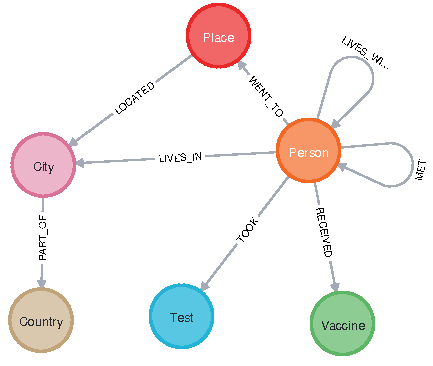
\includegraphics[width=0.95\textwidth]{meta_graph.pdf}
    \caption{Meta graph visualization}
\end{center}
\end{figure}





%===========================================================
%===========================================================

\bibliographystyle{ieeetr}
\bibliography{refs}

\end{document} 
